% This is LLNCS.DEM the demonstration file of
% the LaTeX macro package from Springer-Verlag
% for Lecture Notes in Computer Science,
% version 2.4 for LaTeX2e as of 16. April 2010
%
\documentclass{llncs}
%
\usepackage{makeidx}  % allows for indexgeneration
\usepackage{algorithm}
%\usepackage{algorithmicx}
\usepackage{multirow}
\usepackage{amsmath}
\usepackage{xcolor}
\usepackage{algpseudocode}

\renewcommand{\algorithmicrequire}{\textbf{Input:}}  % Use Input in the format of Algorithm
\renewcommand{\algorithmicensure}{\textbf{Output:}} % Use Output in the format of Algorithm
%
\begin{document}
%
\frontmatter          % for the preliminaries
%
\pagestyle{headings}  % switches on printing of running heads
\addtocmark{Hamiltonian Mechanics} % additional mark in the TOC
%
\chapter*{Preface}
%
This  is intended for use by students of physics, physical
chemistry, and theoretical chemistry. The reader is presumed to have a
basic knowledge of atomic and quantum physics at the level provided, for
example, by the first few chapters in our book {\it The Physics of Atoms
and Quanta}. The student of physics will find here material which should
be included in the basic education of every physicist. This book should
furthermore allow students to acquire an appreciation of the breadth and
variety within the field of molecular physics and its future as a
fascinating area of research.

For the student of chemistry, the concepts introduced in this book will
provide a theoretical framework for that entire field of study. With the
help of these concepts, it is at least in principle possible to reduce
the enormous body of empirical chemical knowledge to a few basic
principles: those of quantum mechanics. In addition, modern physical
methods whose fundamentals are introduced here are becoming increasingly
important in chemistry and now represent indispensable tools for the
chemist. As examples, we might mention the structural analysis of
complex organic compounds, spectroscopic investigation of very rapid
reaction processes or, as a practical application, the remote detection
of pollutants in the air.

\vspace{1cm}
\begin{flushright}\noindent
April 1995\hfill Walter Olthoff\\
Program Chair\\
ECOOP'95
\end{flushright}
%
\chapter*{Organization}
ECOOP'95 is organized by the department of Computer Science, Univeristy
of \AA rhus and AITO (association Internationa pour les Technologie
Object) in cooperation with ACM/SIGPLAN.
%
\section*{Executive Commitee}
\begin{tabular}{@{}p{5cm}@{}p{7.2cm}@{}}
Conference Chair:&Ole Lehrmann Madsen (\AA rhus University, DK)\\
Program Chair:   &Walter Olthoff (DFKI GmbH, Germany)\\
Organizing Chair:&J\o rgen Lindskov Knudsen (\AA rhus University, DK)\\
Tutorials:&Birger M\o ller-Pedersen\hfil\break
(Norwegian Computing Center, Norway)\\
Workshops:&Eric Jul (University of Kopenhagen, Denmark)\\
Panels:&Boris Magnusson (Lund University, Sweden)\\
Exhibition:&Elmer Sandvad (\AA rhus University, DK)\\
Demonstrations:&Kurt N\o rdmark (\AA rhus University, DK)
\end{tabular}
%
\section*{Program Commitee}
\begin{tabular}{@{}p{5cm}@{}p{7.2cm}@{}}
Conference Chair:&Ole Lehrmann Madsen (\AA rhus University, DK)\\
Program Chair:   &Walter Olthoff (DFKI GmbH, Germany)\\
Organizing Chair:&J\o rgen Lindskov Knudsen (\AA rhus University, DK)\\
Tutorials:&Birger M\o ller-Pedersen\hfil\break
(Norwegian Computing Center, Norway)\\
Workshops:&Eric Jul (University of Kopenhagen, Denmark)\\
Panels:&Boris Magnusson (Lund University, Sweden)\\
Exhibition:&Elmer Sandvad (\AA rhus University, DK)\\
Demonstrations:&Kurt N\o rdmark (\AA rhus University, DK)
\end{tabular}
%
\begin{multicols}{3}[\section*{Referees}]
V.~Andreev\\
B\"arwolff\\
E.~Barrelet\\
H.P.~Beck\\
G.~Bernardi\\
E.~Binder\\
P.C.~Bosetti\\
Braunschweig\\
F.W.~B\"usser\\
T.~Carli\\
A.B.~Clegg\\
G.~Cozzika\\
S.~Dagoret\\
Del~Buono\\
P.~Dingus\\
H.~Duhm\\
J.~Ebert\\
S.~Eichenberger\\
R.J.~Ellison\\
Feltesse\\
W.~Flauger\\
A.~Fomenko\\
G.~Franke\\
J.~Garvey\\
M.~Gennis\\
L.~Goerlich\\
P.~Goritchev\\
H.~Greif\\
E.M.~Hanlon\\
R.~Haydar\\
R.C.W.~Henderso\\
P.~Hill\\
H.~Hufnagel\\
A.~Jacholkowska\\
Johannsen\\
S.~Kasarian\\
I.R.~Kenyon\\
C.~Kleinwort\\
T.~K\"ohler\\
S.D.~Kolya\\
P.~Kostka\\
U.~Kr\"uger\\
J.~Kurzh\"ofer\\
M.P.J.~Landon\\
A.~Lebedev\\
Ch.~Ley\\
F.~Linsel\\
H.~Lohmand\\
Martin\\
S.~Masson\\
K.~Meier\\
C.A.~Meyer\\
S.~Mikocki\\
J.V.~Morris\\
B.~Naroska\\
Nguyen\\
U.~Obrock\\
G.D.~Patel\\
Ch.~Pichler\\
S.~Prell\\
F.~Raupach\\
V.~Riech\\
P.~Robmann\\
N.~Sahlmann\\
P.~Schleper\\
Sch\"oning\\
B.~Schwab\\
A.~Semenov\\
G.~Siegmon\\
J.R.~Smith\\
M.~Steenbock\\
U.~Straumann\\
C.~Thiebaux\\
P.~Van~Esch\\
from Yerevan Ph\\
L.R.~West\\
G.-G.~Winter\\
T.P.~Yiou\\
M.~Zimmer\end{multicols}
%
\section*{Sponsoring Institutions}
%
Bernauer-Budiman Inc., Reading, Mass.\\
The Hofmann-International Company, San Louis Obispo, Cal.\\
Kramer Industries, Heidelberg, Germany
%
\tableofcontents
%
\mainmatter              % start of the contributions
%
\title{Hamiltonian Mechanics unter besonderer Ber\"ucksichtigung der
h\"ohreren Lehranstalten}
%
\titlerunning{Hamiltonian Mechanics}  % abbreviated title (for running head)
%                                     also used for the TOC unless
%                                     \toctitle is used
%
\author{Zhimin Wu\inst{1} \and Yang Liu\inst{1}}
%
\authorrunning{Zhimin Wu et al.} % abbreviated author list (for running head)
%
%%%% list of authors for the TOC (use if author list has to be modified)
\tocauthor{Ivar Ekeland, Roger Temam, Jeffrey Dean, David Grove,
Craig Chambers, Kim B. Bruce, and Elisa Bertino}
%
\institute{Princeton University, Princeton NJ 08544, USA,\\
\email{zwu010@e.ntu.edu.sg},\\ WWW home page:
\texttt{http://users/\homedir iekeland/web/welcome.html}
\and
Universit\'{e} de Paris-Sud,
Laboratoire d'Analyse Num\'{e}rique, B\^{a}timent 425,\\
F-91405 Orsay Cedex, France}

\maketitle              % typeset the title of the contribution

\begin{abstract}
The zhimin \dots
\keywords{cs}
\end{abstract}
%
\section{Introduction}
%
%
\section{Counterexample Generation in LTL Model Checking}
%
%
\section{GPU Architecture and CUDA Dynamic Parallelism}\label{sec:sec3}
%
%
\section{CUDA Counterexample Generation}
%
In this chapter, we will describe our CUDA Counterexample Generation proposal. The Key point of Counterexample Generation, as we mentioned, is a BFS-Related Path Generation work. The important properties of a parallel BFS contain the task queue management and the load balance during the search level by level. We take all these into consideration in our design. Based on the CUDA Dynamic Parallelism and GPU programming model, firstly, we propose the overall design of CUDA Counterexample Generation Algorithm. Then we explain in detail about the Two-Level Queue Management and Two-level Task Schedule in our design. Finally we propose the Path Record during the search of counterexample.
%
\subsection{CUDA Dynamic Path Generation Algorithm}
%
The original Counterexample Generation algorithm is shown in \ref{}. To design the CUDA Counterexample Generation proposal, we should focus on the key point, which means CUDA accelerated BFS-related algorithm in GPU. In normal CUDA program, host will call the kernel to run in GPU with static grid and block structure. And in the previous research CUDA IIIT-BFS \ref{}, it need to launch the kernel each time when a level of the graph is explored, which is costly and slower than CPU-BFS. To deal with this problem, research CUDA UIUC-BFS \ref{} propose a hierarchical memory management proposal. It build three level queue for BFS to avoid consequently launch kernel, which result in a certain speedup. But it is still a static method that can not adjust according to the task size; and there is no load balance plan in it. In addition, the above research does not focus on model checking.

There is also some research on BFS-Related CUDA accelerated model checking algorithms.

To deal with these problems. Our solution to CUDA Counterexample Generation is to utilizes new features of CUDA, new GPU architecture and refers to some previous research to do our own expanding. Then we got a new CUDA Path Generation Algorithm to replace the XXX\ref{} in original Counterexample Generation algorithm \ref{}. Totally Speaking, the feature we focus on is he amount of tasks during the execution of BFS is dynamically changing. Our algorithm contains four parts:

\begin{itemize}
    \item We utilize the CUDA Dynamic Parallelism to dynamically fork Child threads to fit the changing of tasks. We build a dynamic Parent-Child relationship.
    \item We build a Three-Level Queue Management proposal to fit the dynamic parallelism and dynamic task expanding.The three-level is made up of two physical level and a virtual level.
    \item We build a Two-level Dynamic Task Schedule to fit the dynamic Parent-Child relationship control and load balance.
    \item We utilize the hierarchical Memory in GPU to do the Two-Level Path Recording and duplicate elimination to some extent.
\end{itemize}

We present the design of our algorithm in Algorithm $1$, Algorithm $2$ and Algorithm $3$: Algorithm 1 propose the \textsl{CudaParentPathGeneration} Algorithm. It is the kernel launched by host.It contains the initial steps of Path Generation and will finish a certain amount of BFS-related tasks. It major focus on the Parent-level task schedule, Queue Management, fork
Child-threads and distributed tasks to them. It controls the Parent-Child Relationship during the execution. Line X to Line X is

            %algorithm1
			\begin{algorithm}[h]
			%\fontsize{9pt}{9pt}\selectfont
			\caption{CudaParentPathGeneration Algorithm}
			\label{alg:PGpath}
			\begin{algorithmic}[1]
            \Require $Start\_ID, SCCnodelist/ACCnodelist, OutgoingRelation$
            \State Define \_shared\_ $S\_queue, Queuesize, Ifexpanded, IfSCC\/AccReach;$ 
            \If{$inblockthreadindex = 0$}
                \State Three-levelQM: $S\_queue.enqueue(Start\_ID)$;
                \State Path-Recording: $path\_record\_queue inside StartNode$;
            \EndIf
            \State $Intra\_block_syn();$
            \While{$Ifexpanded \neq TRUE$}
                \If{$inblockthreadindex < Queuesize$}
                    \State Three-levelQM:$S\_queue.ParallelDequeue()$;\
		            \State CudaScc\&AccReach: $SCC\&AccReach detection$;\
		            \State $BFS, OutgoingRelation \Rightarrow NEXT level$;\
		            \State Path\-Recording:$Inherit\&Update(path\_record\_queue of each Node)$;\
		            \State Three\-levelQM:$S\_queue.ParallelEnqueue()$;
                \EndIf
                \If {$inblockthreadindex == 0$}
                    \State $Queuesize \Leftarrow S_queue.size$;\
		            \If{$Queuesize > THRESHOLD$}
			             \State $Ifexpanded = TRUE$;
                    \EndIf
                \EndIf
            \EndWhile
            \State $Intra\_block_syn()$;
            \If{$inblockthreadindex == 0$}
                \State Prepare for parallelism expanding:
		        \State Two-levelTS: $Parent-level Initial Task Schedule;$
		        \State Three-LevelQM: $Build \_device\_ G_queue;$
                \State $Update(Expanding\_ChildSize), Initial(\_device\_ G\_IfSCC\&AccReach);$
            \EndIf
            \State $Intra\_block_syn();$
            \While{$!IfSCC\&AccReach AND !G_IfSCC\&AccReach$}
	            \If($inblockthreadindex == 0$)
		              \State Three-levelQM: $Build(\_device\_ V\_G\_Queue);$
	                  \State Two-levelTS: $ParellelCal(Child\_Tasks\_Offset\_V\_G\_Queue);$
                \EndIf
	            \If{$inblockthreadindex == 0$}
		              \State Call CudaChildPathGeneration<<<�>>>($V\_G\_Queue,Child\_Tasks\_Offset\_V\_G\_Queue,... $);
                      \State $CudaDeviceSyn():If Childs NOT fit tasks OR finished, return to Parent;$
                      \State $Then Continue loop$:Two-levelTS:$Parent Reschedule tasks, Child re-expanding;$
                \EndIf
	        \EndWhile
            \State $Intra\_block\_syn()$;
            \end{algorithmic}
			\end{algorithm}

Algorithm $2$ propose the \textsl{CudaChildPathGeneration} Algorithm. It is the kernel launched by parent thread, regarded as Child kernel. It will finish the major tasks of Path Generation. It contains the Child-level Queue Management, Child-level task schedule and maintain the Parent-Child Relationship during the execution. Line X

            %algorithm2
            \begin{algorithm}[t]
            \caption{CudaChildPathGeneration Algorithm}
            \label{alg:CGpath}
            \begin{algorithmic}[1]
            \Require
            $\_device\_ V\_G\_Queue, Child\_Tasks\_offset, SCCnodelist\/AccNodelist, OutgoingRelation 
            Pre-define \_device\_ (Child\_Expandedtask, Child\_syn\_need, Child\_need\_back2parent, G\_IfSCC\&AccReach)$
            \State Define \_shared\_ ($Child\_S\_Queue, queuesize, IfSCC\&Accreach);$
            \State Get $inblockthreadindex, globalthreadindex;$
            \If {$inblockthreadindex == 0$)
                \State $Initialize(queensize, IfSCC\&Accreach);$
            \EndIf
            \If {$globalthreadindex == 0$)
                \State $Initialzie(all \_device\_ variables);$
            \EndIf
            \State CudaInterBlockSyn();
            \While {$!G_IfSCC\&AccReach AND !Child_need_back2parent$}
	            \State $BlockTasks = Child\_Tasks\_offset[blockindex + 1] � Taskoffsetsindex[blockindex];$
	            \State Three-levelQM: $Enqueue(Getthreadtask FROM V\_G\_Queue);$
                \State $Queuesize \Leftarrow blocktasks.num;$
                \State $Intra\_block\_syn();$
	            \If {$inblockthreadindex < queuesize$}
		             \State Three-levelQM:$Child\_S_Queue.ParallelDequeue();$
		             \State CudaScc\&AccReach: $SCC\&AccReach detection;$
                            \If {$Reach SCC$}
                                \State $G\_IfSCC\&AccReach = TRUE, Record Path;$
                                \State $BREAK;$
                            \EndIf
		             \State \BFS{}, $OutgoingRelation \Rightarrow NEXT level;$
		             \State $IFDuplicate$ \Leftarrow Path\-Recording:$Inherit\&Update(path\_record\_queue of each Node);$
                            \If {$IFDuplicate == TRUE$}
                                \State $CONTINUE;$
		             \State Three-levelQM:$S\_queue.ParallelEnqueue();$
	            \EndIf
                \State $Intra\_block\_syn();$
	            \If {$inblockthreadindex == 0$}
		             \State $queuesize \Leftarrow Child_S_Queue.size;$
		             \If{$queuesize > block Threshold)$}
			             \State $Child_syn_neede = TRUE;$
                     \EndIf
                \EndIf
	            \State $CudaInterBlocksSyn();$
	            \If {$child_syn_needed == TRUE$}
		            \State Three-levelQM: $Parallel\_Update(G\_Queue)$;
                    \If {$globalthreadindex == 0$}
                        \State $Build(V_G_Queue);$
                        \State Two-levelTS: $Inter\_Childblocks_Tasks_Reschedule;$
            		    \If {$Whole\_blocks\_overloaded$}
			                 \State $Child\_return2Parent = TRUE;$
                        \EndIf
			         \EndIf
                     \State $CudaInterblocksSyn();$
                \EndIf	
            \EndWhile
            \State $CudaInterblocksSyn();$
            \end{algorithmic}
            \end{algorithm}

Algorithm $3$ propose the \textsl{CudaQuicksort},\textsl{Scc\&AccReach} and \textsl{CudaBlocksSyn} Algorithm. \textsl{CudaQuicksort} algorithm utilize the Dynamic Parallelism feature of CUDA to do quick sort for SCC node list.This refer to \ref{}. \textsl{Scc\&AccReach} use the Binary search to find if the path generation execution has reached SCC. \textsl{CudaInterBlocksSyn} Algorithm refers to the algorithm mentioned in \ref{}. It choose the \textsl{simple\_blocks\_synchronize} when the number of blocks is small. And the \textsl{tree\_blocks\_synchronize} is for large number of blocks.

            %algorithm 3
            \begin{algorithm}[t]
            \caption{CudaQuicksort, Scc\&AccReach and CudaInterBlocksSyn Algorithm}
            \label{alg:Algmulti}
            \begin{algorithmic}[1]
            \State CudaQuickSort($data, pivot, left, right$)
                \State Define $nleft$,$nright$;
                \State $Partition(data+left, data+right, pivot, nleft, nright);$
                \If {$left < nright$}
                    $CreatCudastream(s1);$
                    $CudaQuickSort<<<...s1>>>(data, left, nright);$
                \EndIf
                \If {$nleft < right$}
                    $CreateCudasteam(s2);$
                    $CudaQuickSort<<<...s2>>>(data, nleft, right);$
                \EndIf
                \\
            \State Scc\&AccReach()
                \State $Normal Binary Search$ \\
                \\
            \State CudaInterBlocksSyn()
                \If {$blocks.num < THRESHOLD$}
                    $simple\_blocks\_synchronize();$
                \Else
                    $tree\_blocks\_synchronize();$
                \EndIf
            \end{algorithmic}
            \end{algorithm}

From the overall introduction of algorithms, the structure of our solution to the CUDA counterexample generation is clearly. Totally speaking, we utilize the dynamic parallelism technique from latest CUDA. But the key point is that we finish a complete scheme to make our algorithm available to utilize this support from cuda, as well as fit the new GK110 architecture. Then we reach the ultimate goal of working out a novel CUDA counterexample generation scheme. In the following parts, more detail will be introduced.
%
\subsection{Dynamic Parent-Child Relationship}
%
Data-dependent parallel work can be generated inline with CUDA Dynamic Parallelism\ref{}. So building the relationship between \textsl{Parent} and \textsl{Child} is a data-driven work. In our algorithm design, in order to maximize the utilization of parallelization, each thread is asked to just do the breadth search and path recording of one node. It means the number of nodes in each level of BFS will decide the needed threads number. Therefore, with the node number uncertainty in BFS-related Path Generation, the best way is to allocate threads during runtime. That is what our algorithms do. And in order to save the cost, our \textsl{Parent}, which is launched by host, should not be a large scale grid. The major tasks of path generation should be done by \textsl{Child} and the \textsl{Parent} focus on the initial steps of path generation and the \textsl{Parent-Child} relation management. In our algorithm, \textsl{Parent} will always be just one \textsl{block}. As the minimum source schedule unit in GPU is \textsl{warp}, the GK110 can support \textsl{$4$ warps} running at the same time, we always choose $4-warps\times\alpha$ as the threads number of \textsl{Parent} grid.

We show the relationship in \ref{fig:PCRelation}, The \textsl{Parent-Child} relationship is not static. when \textsl{Parent} launch \textsl{Child}, it will base on the current tasks to decide the structure of \textsl{Child}, the future tasks can not be forecasted but it is certainly that \textsl{Parent} should not set a very huge \textsl{Child} grid to prevent task overload. So in most case, \textsl{Parent-Child} relationship is dynamically adjusted. In our algorithm, when the total tasks overload in \textsl{Child},it should return to \textsl{Parent} for reallocating(shown in \ref()). However, launch \textsl{Child} for a lot of time is also costly. so we should make a compromise.It will be mentioned in the Dynamic Two-level Task Schedule part.

\begin{figure}
    \vspace{2.5cm}
    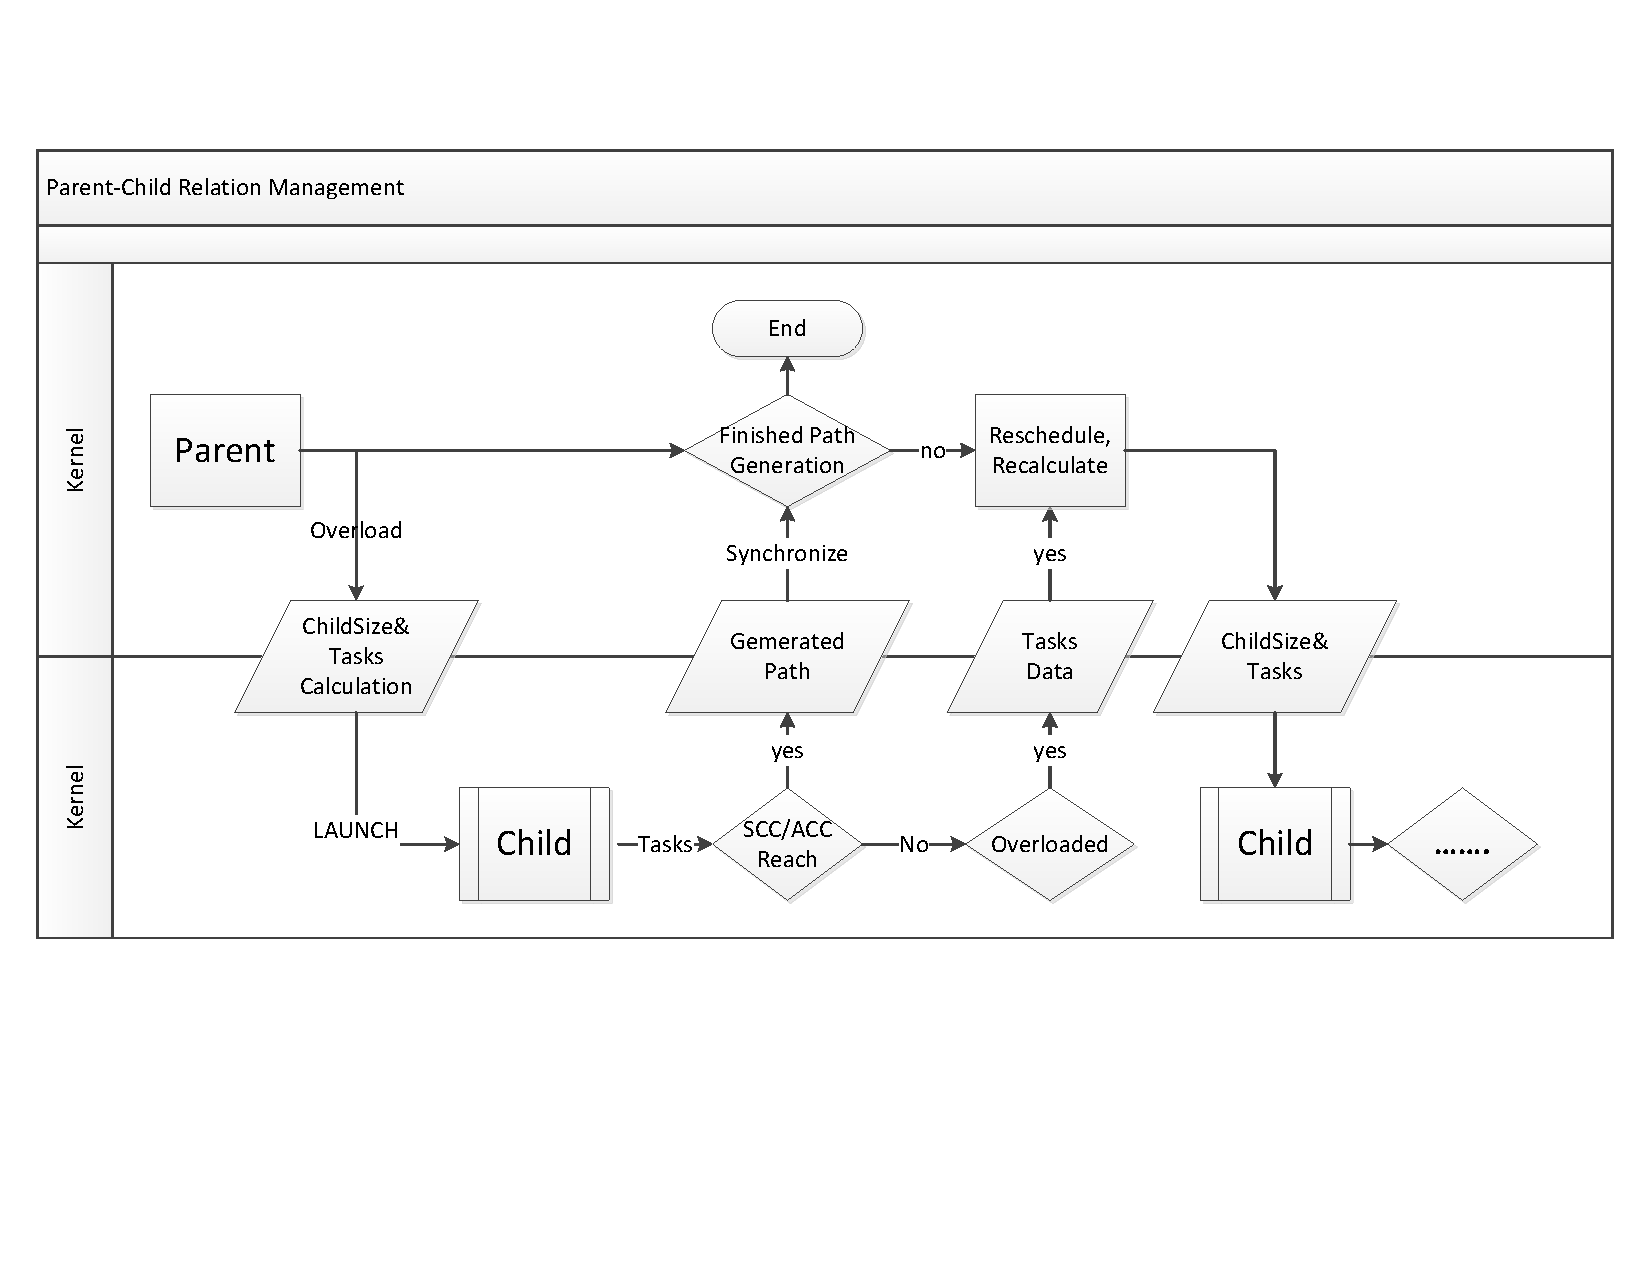
\includegraphics[height=4]{PCRelation.pdf}
    \caption{Parent-Child Relationship}
    \label{fig:PCRelation}
\end{figure}

Beside the total tasks overload in \textsl{Child}, when the \textsl{generated path} in any thread in \textsl{Child} reach the SCC\/ACC ($SCCnodelist\\Accnodelist \cup Nodelist_in_path \neq \emptyset$), all threads in \textsl{Child} should synchronize and send result to \textsl{Parent}. As we mentioned in section XXX, The only way of communication between \textsl{Parent} and \textsl{Child}, as well as among \textsl{Childblocks} is on \textsl{Global Memory}, so the thread that find SCC-reach will record the generated path and a mark in \textsl{Global Memory} then synchronise among all Child blocks. As a result, \textsl{Parent} will got the mark and result and exit the execution.

In total, The \textsl{Parent-Child} relationship is dynamic according to the task overload and SCC Reach. This is very flexible and can fully utilize the dynamic parallelism.It makes our CUDA Path Generation a on-the-fly algorithm.
%
\subsection{Dynamic Three-level Queue Management}
%
As we mentioned in \ref{sec:sec3}, the architecture of Memory in GPU contains Global memory and Shared Memory. Global memory can be read\/write by all blocks running in all SM and Shared Memory is just available to blocks in same SM. Read\/Write operation in Shared Memory cost much less than operation in Global Memory. We should utilize this feature to improve the performance of our algorithm. But the size of shared memory is much lower than Global Memory. For our algorithm that refer to huge data size, we can not get rid of visiting Global memory. Considering the point in dynamic parallelism that only when tasks overload then call Child, we build a dynamic hierarchical Queue to utilize the hierarchical memory. In order to fit our dynamic parallelism design, we build a Three-Level Queue Management scheme. The structure can be shown in \ref{fig:DQM}

\begin{figure}
    \vspace{2.5cm}
    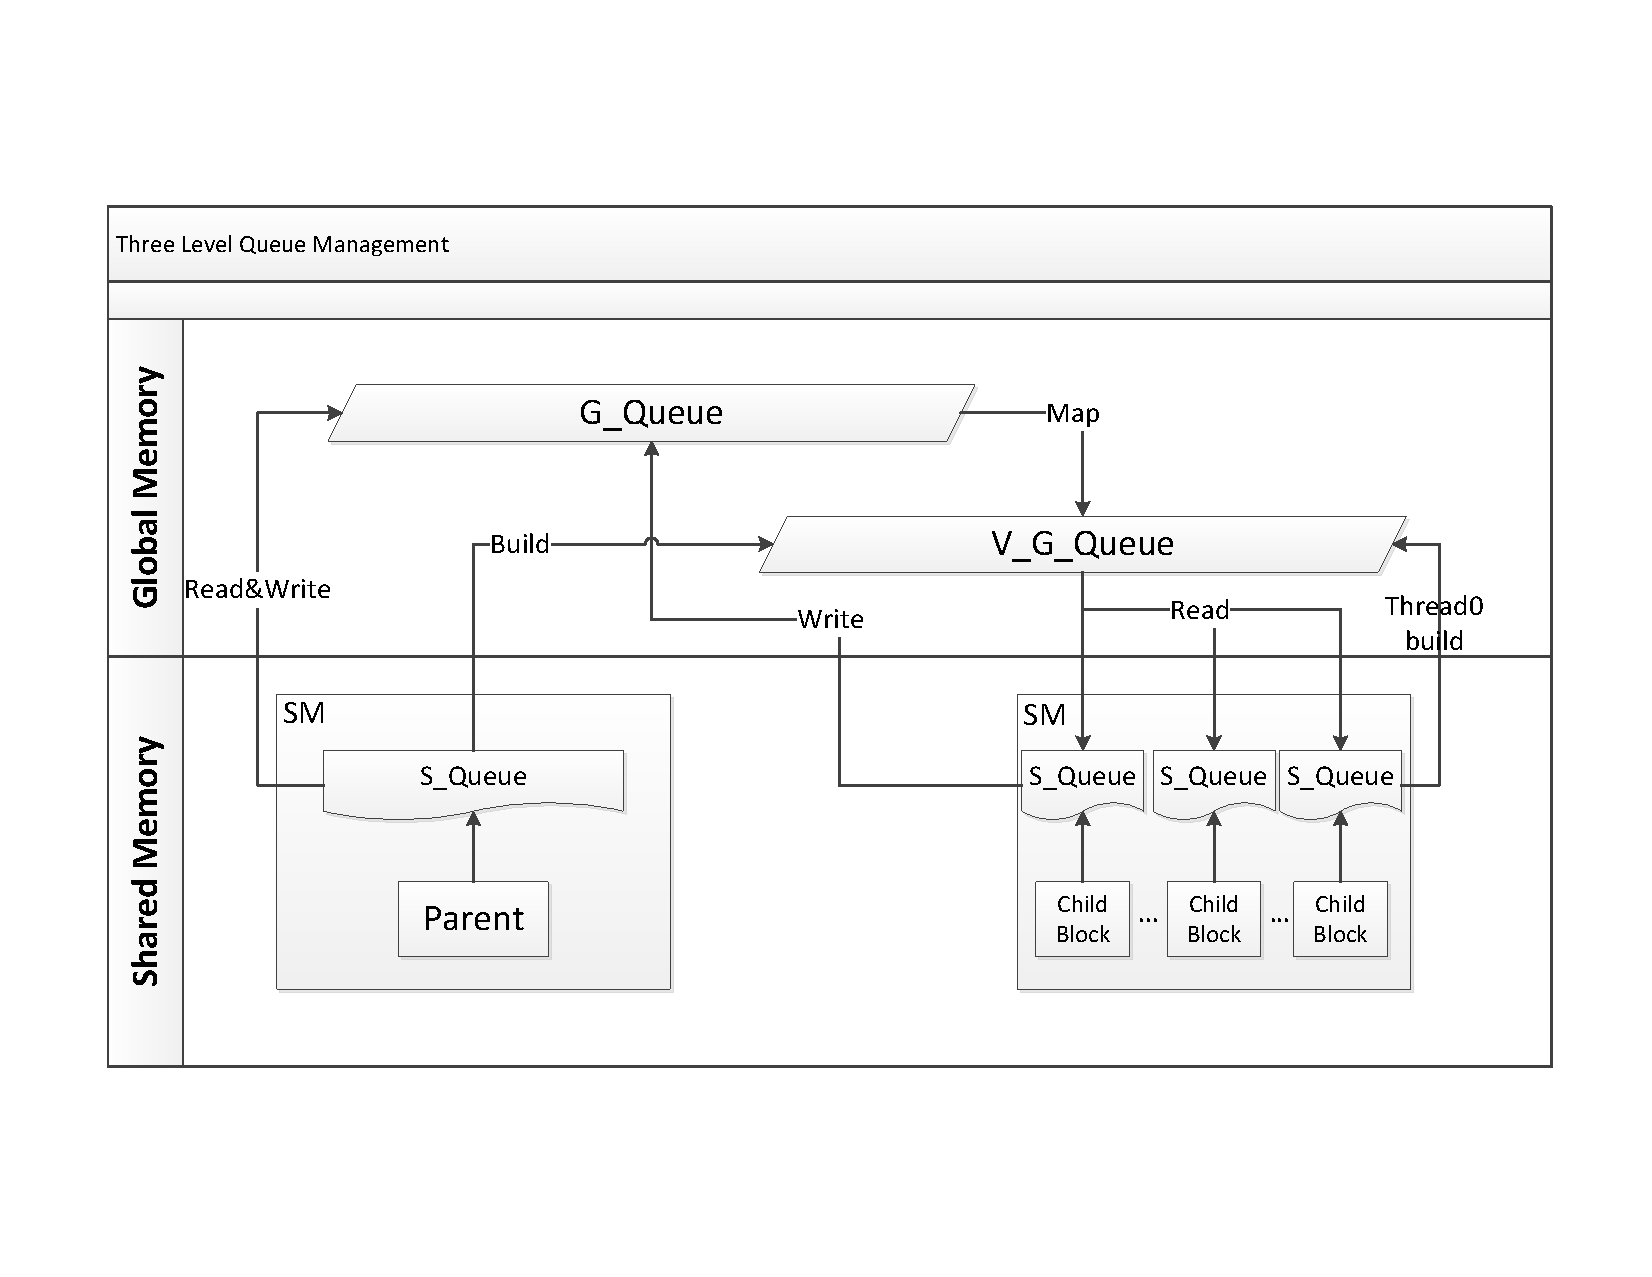
\includegraphics{DQM.pdf}
    \caption{Dynamic Three-level Queue Structure}
    \label{fig:DQM}
\end{figure}

The first level queue is stored in Shared Memory, marked as \textsl{S\_Queue}, It is shared among blocks in 1 SM. The second level queue is stored in Global Memory, marked as \textsl{G\_Queue}. The third level queue is also stored in Global Memory, called Virtual Global Queue, marked as \textsl{V\_G\_Queue}.

\textsl{S\_Queue} is the first task storage queue. When the BFS-related path generation begin, the expanded node ID will firstly be pushed into the \textsl{S_Queue} in corresponding SM. Then for the next level expanding, threads do not need to visit Global Memory, it improve the data access speed. Here, the problem is it may cause read\/write conflict when parallel threads write/read at the same time. Then if we set lock or use atomic operation to prevent conflict, it will cost much with frequently write request at the same time. So based on the GPU SM architecture and new Warp schedule in GK110,we build the lock-free \textsl{S_Queue} in structure showed in \ref{fig:SQueue}. As mentioned, the kernel is actually executed in groups of $32$ threads,called a \textsl{warp}. In GK110, it can support $4$ \textsl{warps} executing at the same time in reality. So for each block, we make the \textsl{S_Queue} a four queue-group with $32$ queues each. So even the threads executed in a SM is much more than 4 \textsl{warps}, the number to write into queue at the same time is limited. \textsl{S_Queue} is the queue directly accessed by threads during execution. As one thread only hold 1 task in each level search, if the tasks in \textsl{S_Queue} exceed the number of threads executed in one block, the tasks should be re-scheduled and then it need to be transferred to \textsl{G_Queue} in Global Memory.

\begin{figure}
    \vspace{2.5cm}
    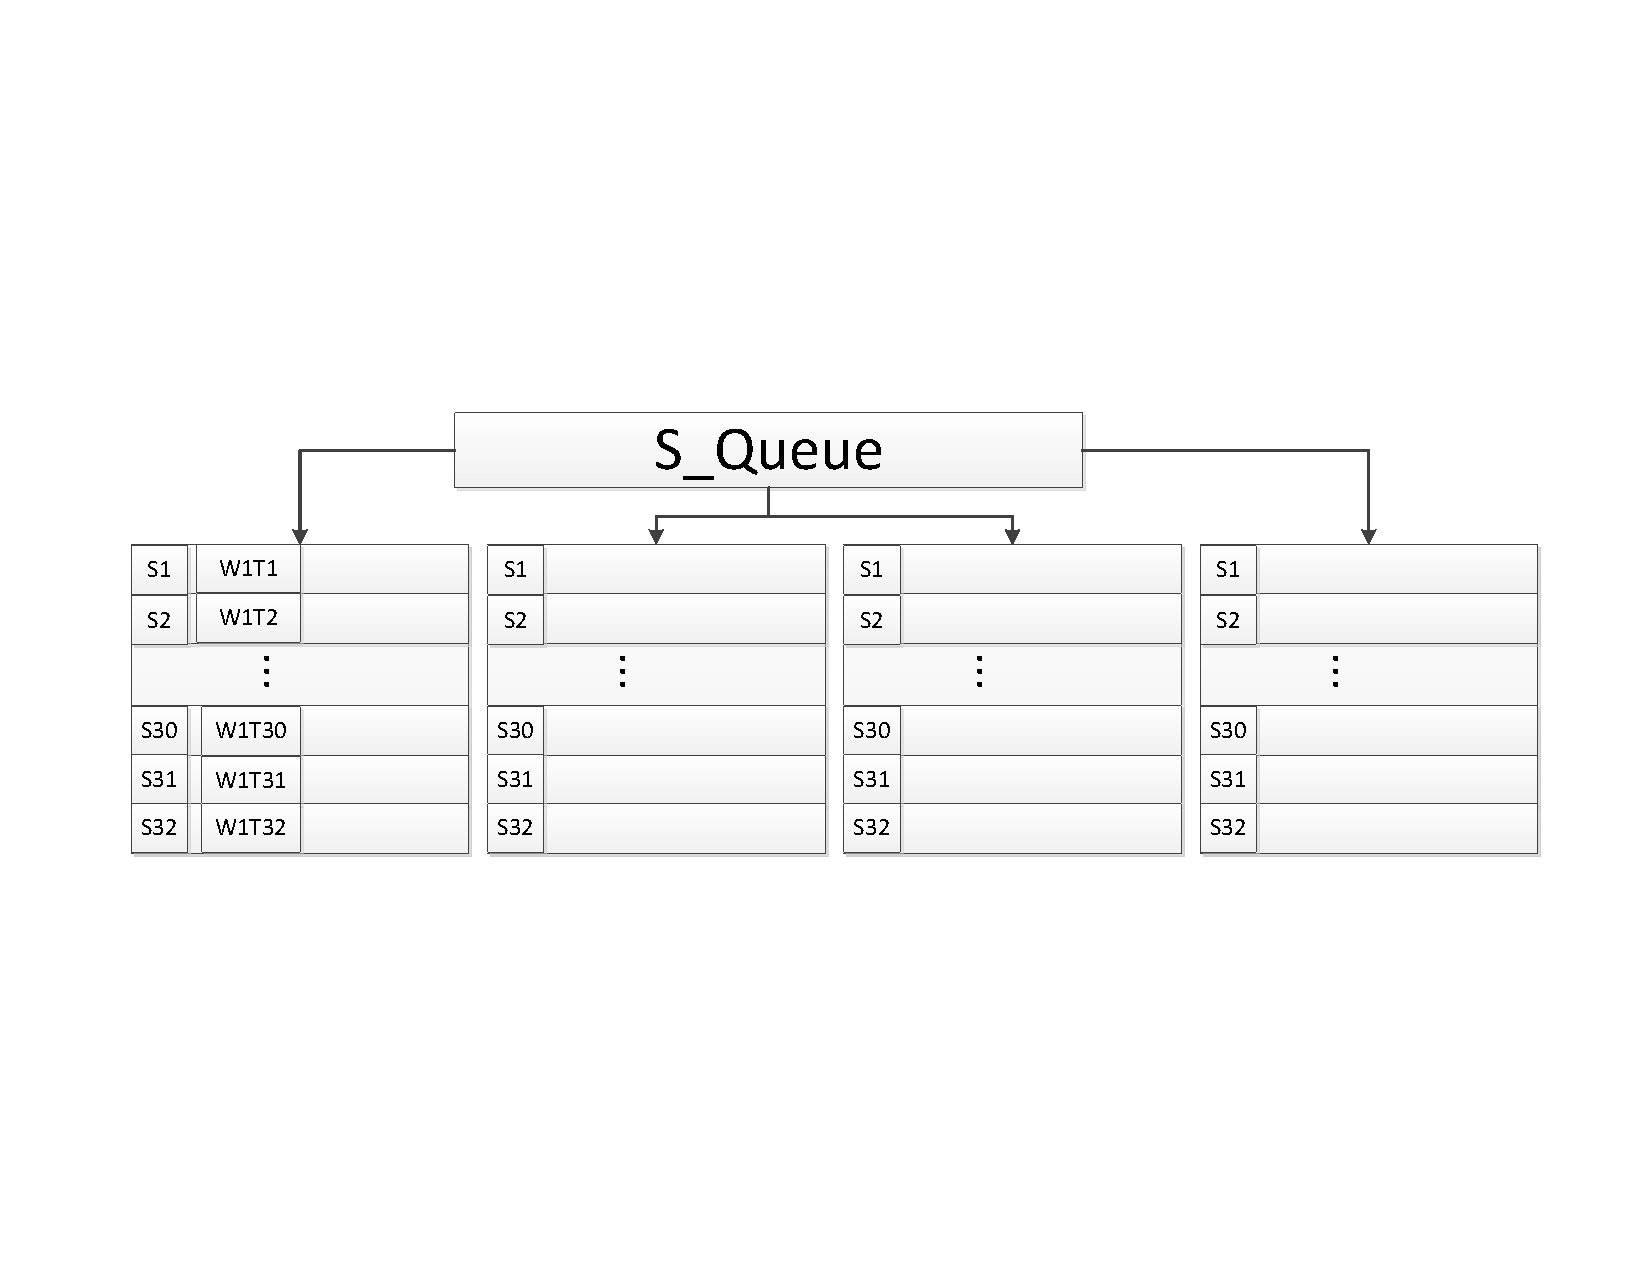
\includegraphics[height=4]{SQueue.pdf}
    \caption{}
    \label{fig:SQueue}
\end{figure}

\textsl{G_Queue} is build at the first time \textsl{Parent} call \textsl{Child}, it is a group of array. As dynamic allocate memeory and visit global memory is costly, this queue won't change after being build. As Global Memory is the way \textsl{Parent} communicate with \textsl{Child},it work as the way to transfer tasks to \textsl{Child} when the first time launching \textsl{Child}. Then in following execution, it stores the tasks when blocks overload and copy the content in \textsl{S_Queue} to it. It is only visible for writing and \textsl{Child} threads will never directly read from it. The way to write \textsl{G_Queue} is shown in \ref{fig:GQueue}.

\begin{figure}
	\vspace{2.5cm}
    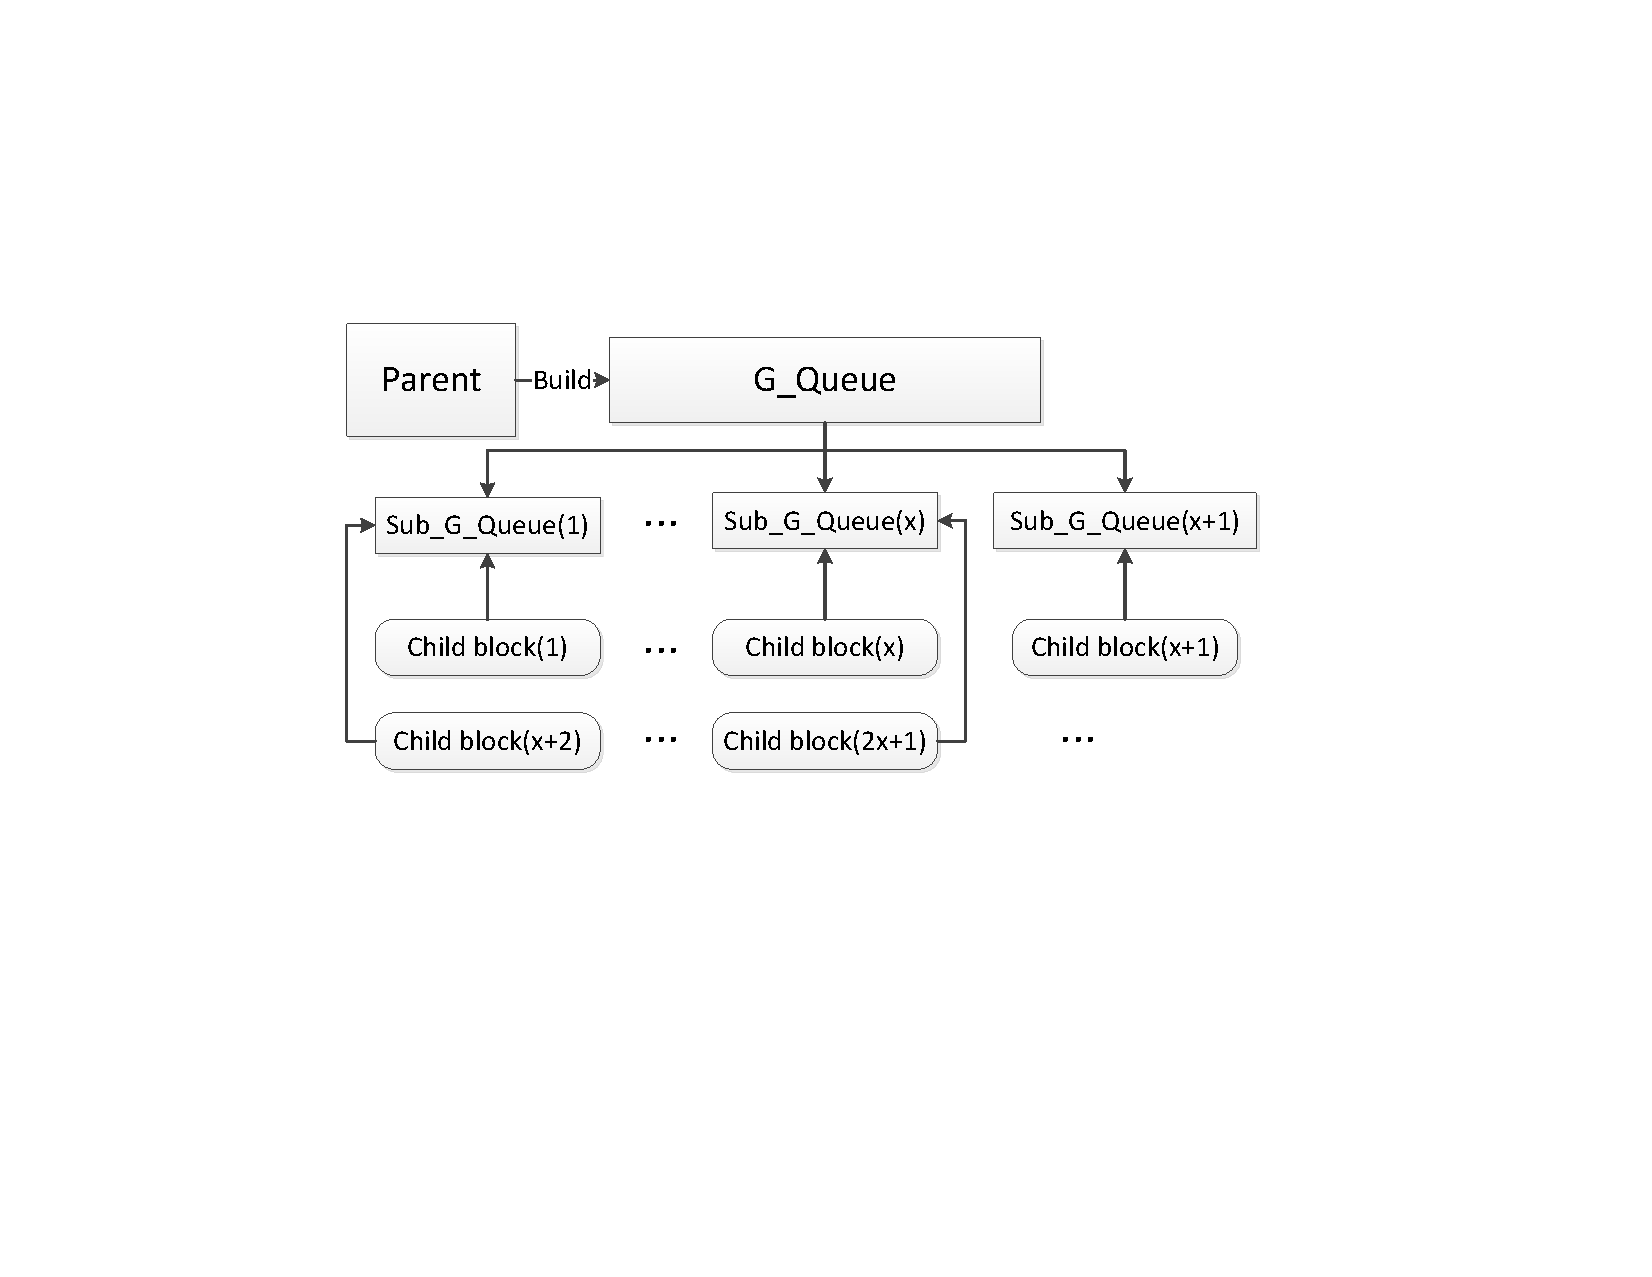
\includegraphics[height=4]{GQueue.pdf}
	\caption{}
	\label{fig:GQueue}
\end{figure}

The Virtual Global Queue is the third level and it is a pointer array. As shown in \ref{flg:VGQueue}, in global view, the tasks store in the \textsl{G_Queue} is not continuous. So it is not convenient for tasks reschedule as it will request a lot of computing on the task range for each thread. Then \textsl{V_G_Queue} is to build a continuous list for task schedule. It is only visible for reading by threads. And only \textsl{V_G_Queue} is dynamic built during execution. It can be shown in \ref{fig:VGQueue}.

\begin{figure}
	\vspace{2.5cm}
    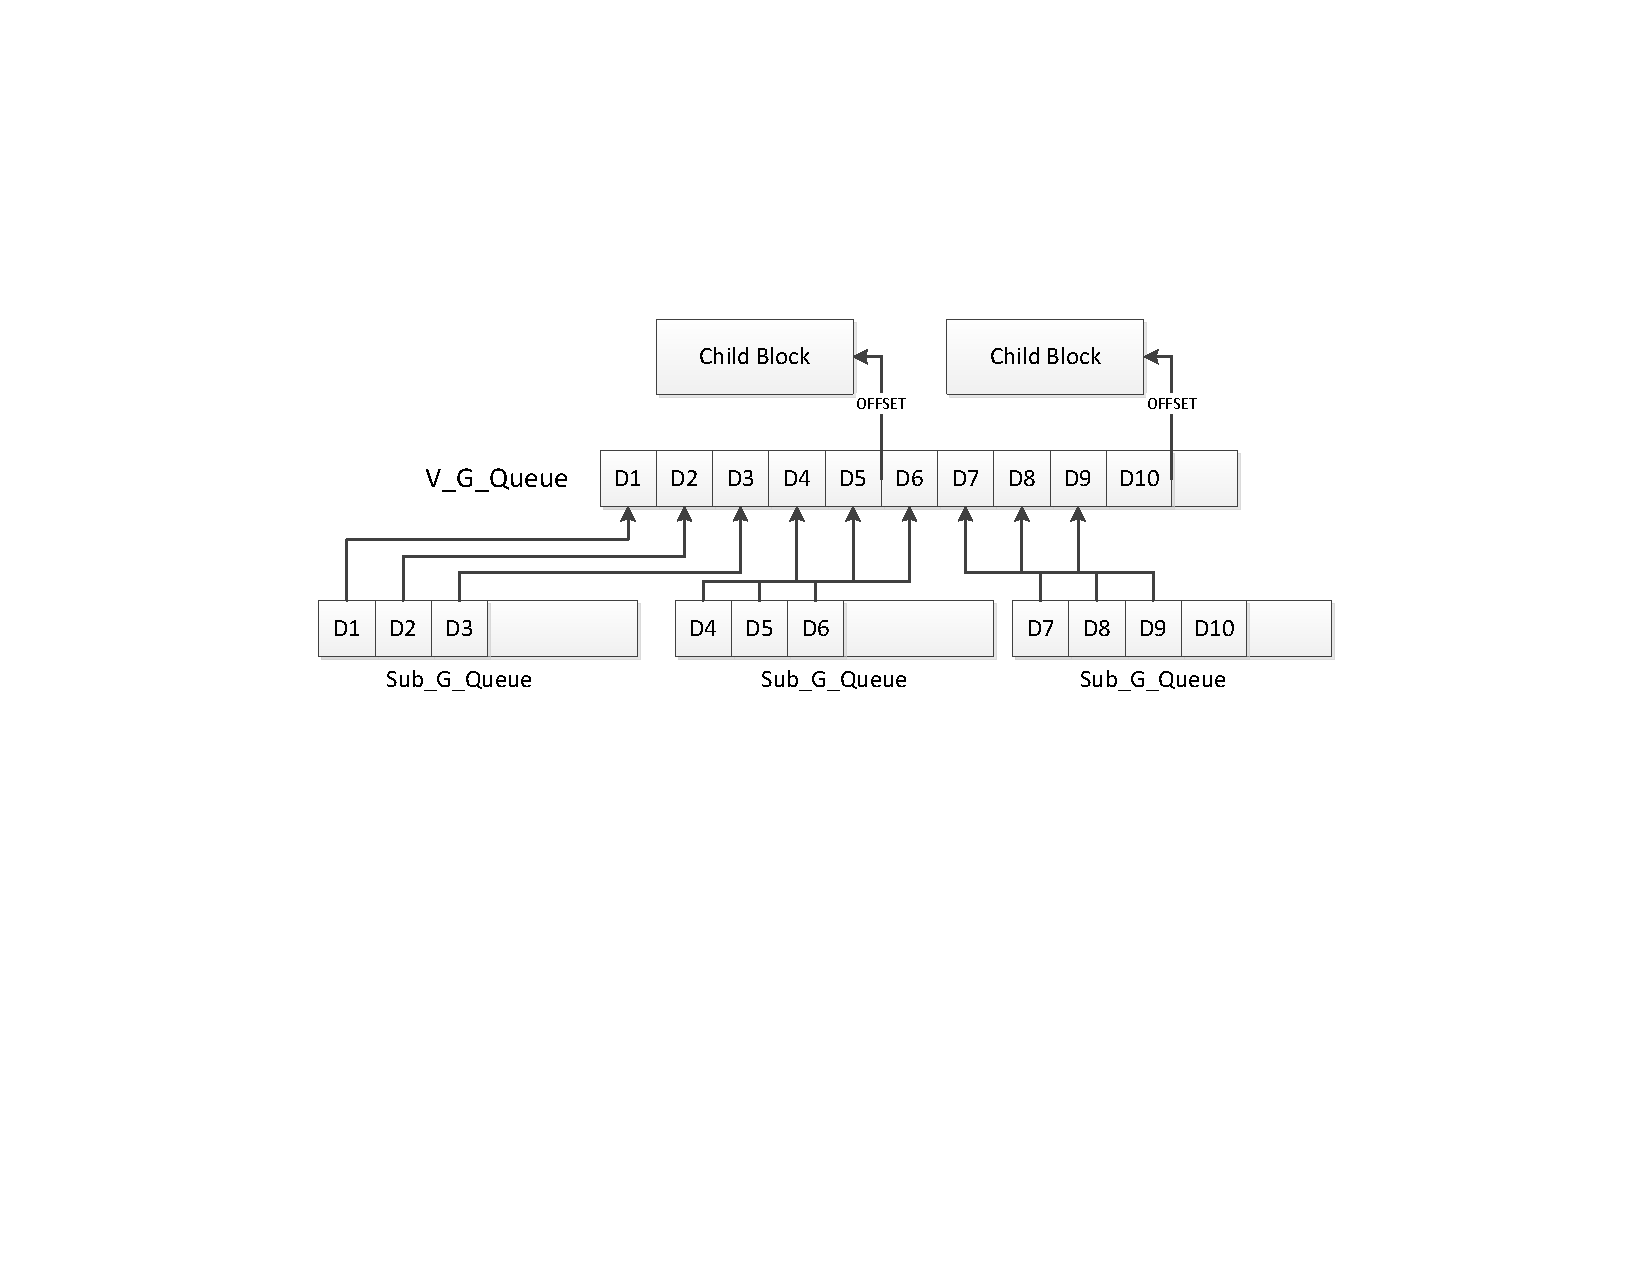
\includegraphics[height=4]{VGQueue.pdf}
	\caption{}
	\label{fig:VGQueue}
\end{figure}

This three-level Queue follows the rules of dynamic parallelism, aiming at building a flexible way of data access and improving the performance. It can work well with the \textsl{Parent-Child} structure.
%
\subsection{Dynamic Two-level Task Schedule}
%
In previous sections, what we mentioned contains two conditions that program need to do task reschedule:
   \begin{itemize}
        \item when \textsl{Parent} finish some initial steps of BFS-related path generation and can not hold more tasks, it need to call \textsl{Child} and schedule tasks to \textsl{Child} the first time.
        \item when the whole tasks make \textsl{Child} blocks overloaded, it need to return to \textsl{Parent} to rearrange the \{Child} grid so as to reschedule the tasks
   \end{itemize}

In this two conditions, tasks schedule is done by \textsl{Parent}. And launching kernel is an expensive work. If just one or a few blocks in \textsl{Child} is overloaded, it is obviously that the execution should not return to \textsl{Parent}. Instead, inside the \textsl{Child}, it should also have a \textsl{Child level inter blocks} task schedule. That, combined with the \textsl{Parent} level task schedule, we build the two-level task schedule. It can be shown in \ref{fig:TwoTS}.

\begin{figure}
    \vspace{2.5cm}
    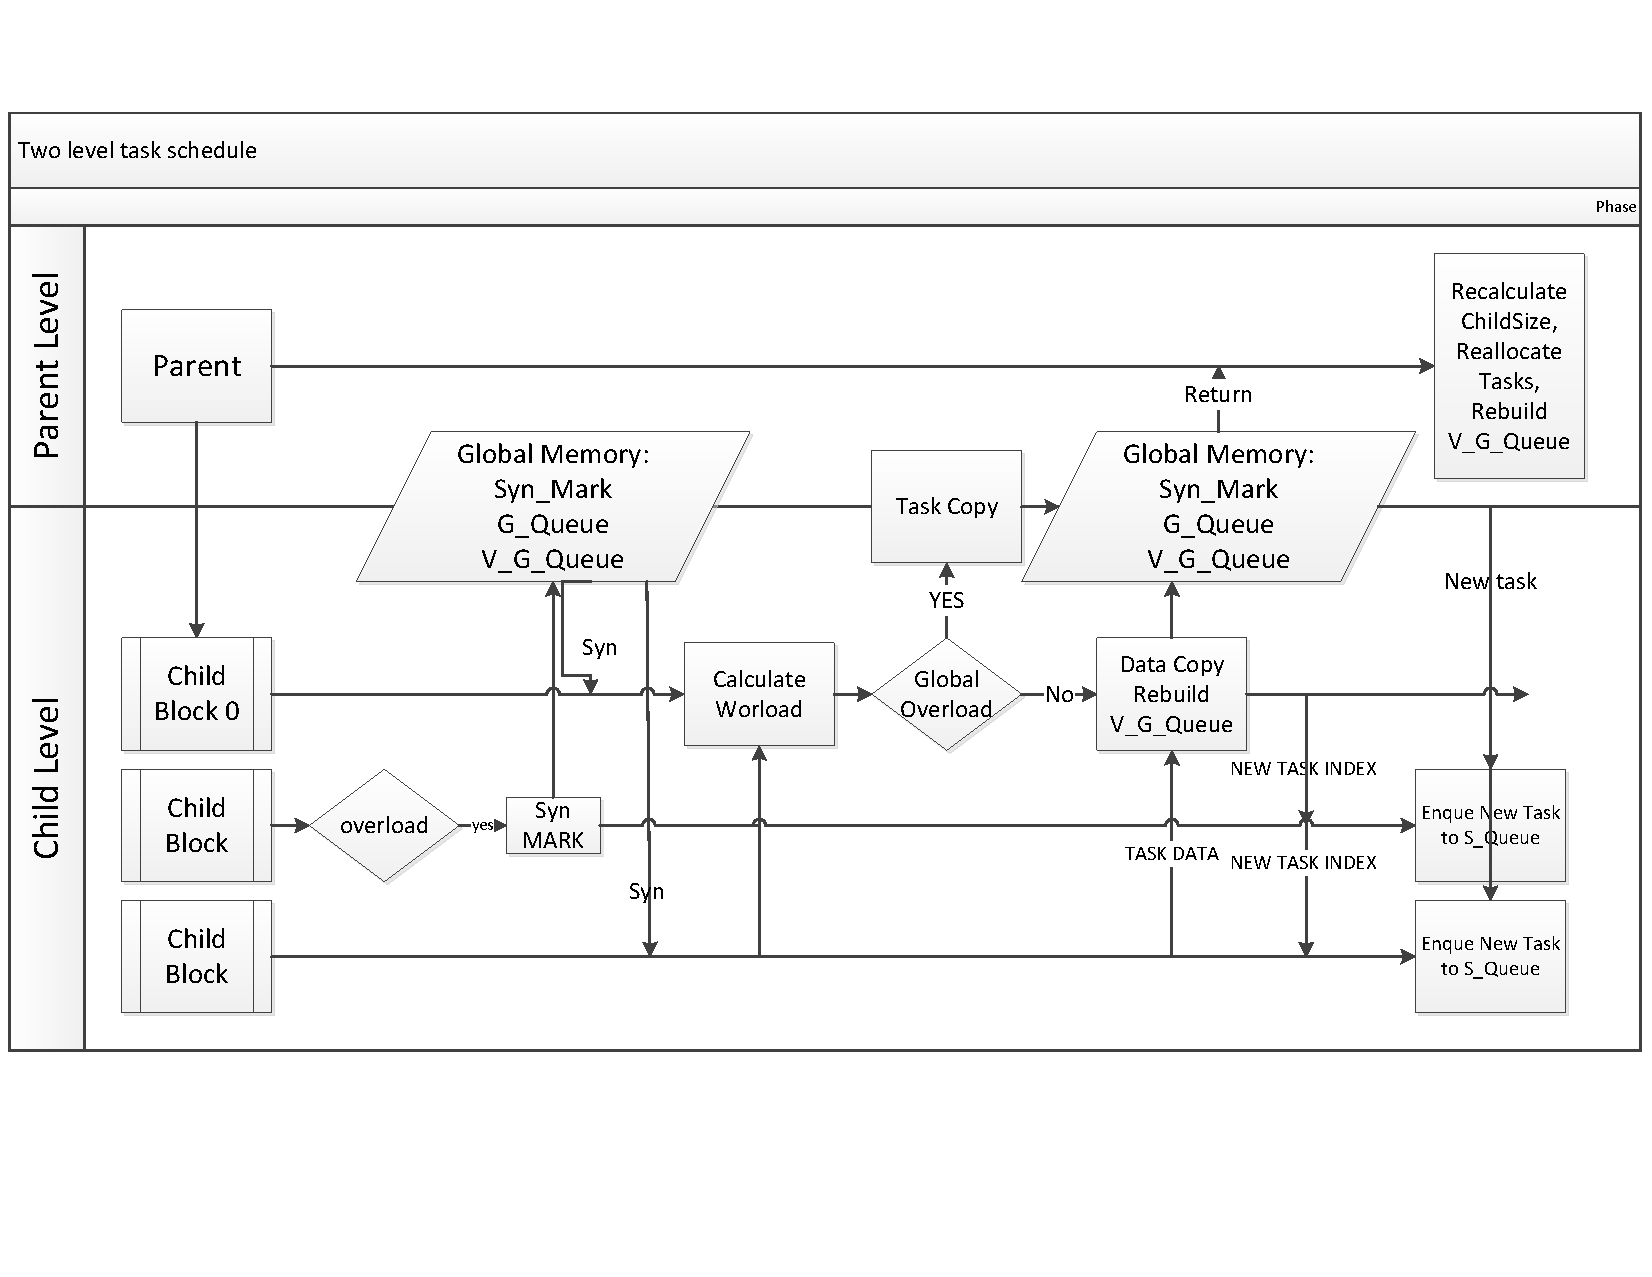
\includegraphics[height=4]{TwoTS.pdf}
    \caption{Dynamic Two-level Task Schedule}
    \label{fig:TwoTS}
\end{figure}

In \textsl{Child} blocks, after each level of path generation, each block will decide if overloaded. Then if so, block will copy tasks in its own \textsl{S_Queue} back to \textsl{G_Queue}. Then mark \textsl{Child_syn_needed} in order to make all other blocks enter the \textsl{Child level} tasks schedule. In our algorithm, the \textsl{Child level} tasks schedule will balance the tasks among all blocks by build new \textsl{V_G_Queue}. This behavior has no reference to \textsl{Parent}. Here, in order to make each block has enough resource to do future expanding, the schedule should not make the new tasks in each block exceed a \textsl{threshold}, Or the algorithm will conclude that the \textsl{Child} is overloaded.

Then it will come to \textsl{Parent level} task schedule. \textsl{Parent} will calculate new \textsl{Childsize-Child blocks number}, build new \textsl{V_G_Queue} and calculate tasks offset for each \textsl{Child block}. Here it also comes to the problem that if \textsl{Childsize} is not appropriate, then the \textsl{Child} will return to \textsl{Parent} frequently, which is costly. To make a compromise, in operation line X in our algorithm, when calculating the \textsl{Childsize}, we guarantee that tasks allocated to each Child should not beyond the number $\textsl{warpsize = 32}$ and the threads number in each \textsl{Child block} should be $warpsize\times\alpha$.
%
\subsection{Two-level Path Recording and Duplicate Elimination}
%
Our algorithm is to deal with the Path Generation so as to get Counterexample. So path recording is necessary. Since the path generation is a BFS-related work, the path record is updated in each search level. Take \ref{fig:PathRExp} as an example, the nodes in each level will inherit their precusor's path and then add themselves in the path. When a node has more than one precursor, it will inherit more than one path. However, our algorithm is to find a path to reach $SCC\/ACCnodelist$, only to inherit one path is enough and this will save the storage space. Then we build the Path Recording scheme according to this and also the dynamic parallelism feature inclued in all other parts.

\begin{figure}
	\vspace{2.5cm}
    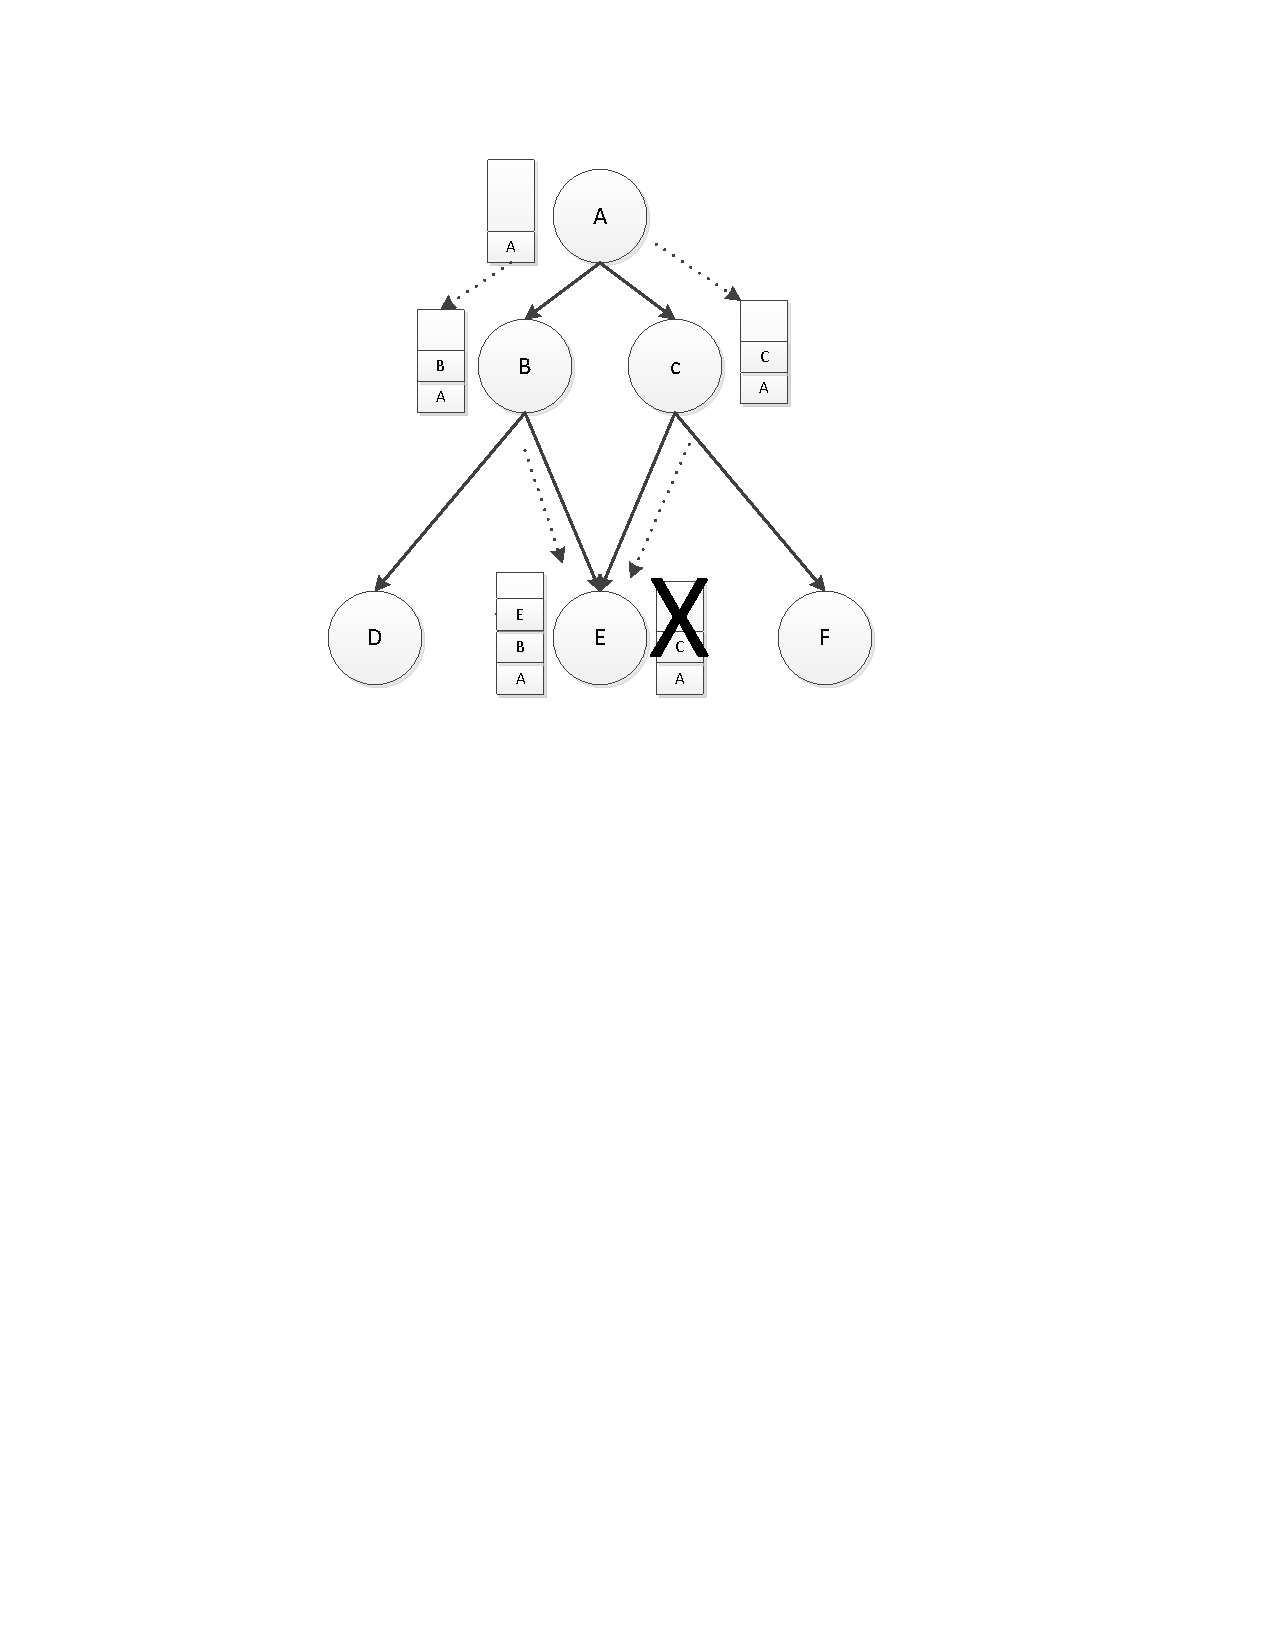
\includegraphics[height=4]{PathRExp.pdf}
	\caption{}
	\label{fig:PathRExp}
\end{figure}

We call our scheme \textsl{Two-level Path Recording}. One is Shared Memory level path recording and the other is Global Memory level. Firstly, a simple structure is defined:

\begin{center} $PathRecordNode{nodeid, pathqueue}$\end{center}

Then we define a \textsl{PathRecordNodeList} array in each block that stored in Shared Memory (called \textsl{S_PRN_List}) and one more array in Global Memory (called \textsl{G_PRN_List}. On a whole, during the path generation, threads will update the path in corresponding node in Shared Memory following the inherit rules mentioned. And the updating of path in Global Memory happens when the overload happens in order to fit the dynamic tasks schedule design previously mentioned. In details, the steps to do the path recording are as follows, all these steps are executed after the \textsl{IfReachSCC\&ACC} detection of current visiting node:

\begin{itemize}
	\item when a node is being visited, update the corresponding \textsl{PathRecordNode} in the \textsl{S_PRN_List} by push itself to the path
	\item when a node is being visited, copy its updated path to each of its successor's corresponding path queue If it is empty. If not, it means the successor has inherit a path and there is no need to inherit another path. Here, it also means the successor has been put into task queue and it can eliminate the duplication inside a block to some extent
	\item when overload happen, we do the path copy together with copy tasks from \textsl{S_Queue} to \textsl{G_Queue}. Only the path data that with ID contained in \textsl{S_Queue} are copied. Here, with the same rule, if the corresponding \textsl{PathRecordNode} has unempty path queue, the copy operation will be aborted and this node ID will also be aborted in task copy. 
	\item these steps continue until \textsl{IfSCC\/ACCReach} detection return TRUE.
\end{itemize}

Here, the reason we say it can just eliminate duplication to some extent is that after once \textsl{S_PRN_List \Rightarrow G_PRN_List} copy, All path queue in \textsl{S_PRN_List} will be empty. So in following steps, the visited node may have possibility to be visited again and it will store the path again. But when copy back to \textsl{G_PRN_Queue}, this will be detected.

Another problem is the storage space problem. (need expanding)

In addition, when a thread updating the path queue in \textsl{PathRecordNode}, atomic operation is needed to prevent conflict. And it should not block other threads. This will be discussed in the following part.
%
\subsection{Synchronization and Atomic Operation}
%
In our algorithm, synchronization contains two parts: intra block synchronization and inter block synchronization. For all threads inside a block, the intra block synchronization should be taken in each level expanding as the algorithm need to judge if overload happen. What we should focus is the inter block synchronization. It requires all blocks to wait until all reach the synchronize point, it will reduce the performance. So inter block synchronization is taken only when necessarily needed. In our Algorithm, the data that blocks in \textsl{Child} need to communicate with each other contains \textsl{IfSCC\/AccReach, If overload and If_return2Parent}. These are stored in Global Memory and will be checked by each thread in each level expanding. If the corresponding event happens being detected by any thread, it will utilize atomic operation to update the data in Global Memory and then called the \textsl{CudaInterBlocksSyn}. After other blocks detect the update, they will also call \textsl{CudaInterBlocksSyn} so as to synchronise among all blocks. 

Here we mention the atomic operation. It is used to build a unblock lock. When some threads want to write the same memory address at the same time, only the first one call the lock will get the access right and the other will abort their write operation and continue their executing. The design of this lock is shown in \ref{alg:atomiclock}

\begin{algorithm}[t]
\caption{Unblock lock with atomic operation}
\label{alg:atomiclock}
\While {$Iffinished == TRUE$}
    \If {$Atomic(&mutex, 1)$}
        \State write operation;
        \State $Iffinished = True$;
        \State $Atomic(&mutex, 0)$;
    \Else
        \State $abort = TRUE$;
        \State break;
    \EndIf
\EndWhile
\end{algorithmic}
\end{algorithm}

With all these above, we build the complete CUDA Path Generation algorithm for Counterexample Generation. All content make full use of the dynamic parallelism and the feature of new Kepler $GK110$ architecture. 
%
\section{Implementation of Algorithm in PAT}
%

%
\section{Experiments and Evaluation}

\section{Fixed-Period Problems: The Sublinear Case}
%
With this chapter, the preliminaries are over, and we begin the search
for periodic solutions to Hamiltonian systems. All this will be done in
the convex case; that is, we shall study the boundary-value problem
\begin{eqnarray*}
  \dot{x}&=&JH' (t,x)\\
  x(0) &=& x(T)
\end{eqnarray*}
with $H(t,\cdot)$ a convex function of $x$, going to $+\infty$ when
$\left\|x\right\| \to \infty$.

%
\subsection{Autonomous Systems}
%
In this section, we will consider the case when the Hamiltonian $H(x)$
is autonomous. For the sake of simplicity, we shall also assume that it
is $C^{1}$.

We shall first consider the question of nontriviality, within the
general framework of
$\left(A_{\infty},B_{\infty}\right)$-subquadratic Hamiltonians. In
the second subsection, we shall look into the special case when $H$ is
$\left(0,b_{\infty}\right)$-subquadratic,
and we shall try to derive additional information.
%
\subsubsection{The General Case: Nontriviality.}
%
We assume that $H$ is
$\left(A_{\infty},B_{\infty}\right)$-sub\-qua\-dra\-tic at infinity,
for some constant symmetric matrices $A_{\infty}$ and $B_{\infty}$,
with $B_{\infty}-A_{\infty}$ positive definite. Set:
\begin{eqnarray}
\gamma :&=&{\rm smallest\ eigenvalue\ of}\ \ B_{\infty} - A_{\infty} \\
  \lambda : &=& {\rm largest\ negative\ eigenvalue\ of}\ \
  J \frac{d}{dt} +A_{\infty}\ .
\end{eqnarray}

Theorem~\ref{ghou:pre} tells us that if $\lambda +\gamma < 0$, the
boundary-value problem:
\begin{equation}
\begin{array}{rcl}
  \dot{x}&=&JH' (x)\\
  x(0)&=&x (T)
\end{array}
\end{equation}
has at least one solution
$\overline{x}$, which is found by minimizing the dual
action functional:
\begin{equation}
  \psi (u) = \int_{o}^{T} \left[\frac{1}{2}
  \left(\Lambda_{o}^{-1} u,u\right) + N^{\ast} (-u)\right] dt
\end{equation}
on the range of $\Lambda$, which is a subspace $R (\Lambda)_{L}^{2}$
with finite codimension. Here
\begin{equation}
  N(x) := H(x) - \frac{1}{2} \left(A_{\infty} x,x\right)
\end{equation}
is a convex function, and
\begin{equation}
  N(x) \le \frac{1}{2}
  \left(\left(B_{\infty} - A_{\infty}\right) x,x\right)
  + c\ \ \ \forall x\ .
\end{equation}

%
\begin{proposition}
Assume $H'(0)=0$ and $ H(0)=0$. Set:
\begin{equation}
  \delta := \liminf_{x\to 0} 2 N (x) \left\|x\right\|^{-2}\ .
  \label{eq:one}
\end{equation}

If $\gamma < - \lambda < \delta$,
the solution $\overline{u}$ is non-zero:
\begin{equation}
  \overline{x} (t) \ne 0\ \ \ \forall t\ .
\end{equation}
\end{proposition}
%
\begin{proof}
Condition (\ref{eq:one}) means that, for every
$\delta ' > \delta$, there is some $\varepsilon > 0$ such that
\begin{equation}
  \left\|x\right\| \le \varepsilon \Rightarrow N (x) \le
  \frac{\delta '}{2} \left\|x\right\|^{2}\ .
\end{equation}

It is an exercise in convex analysis, into which we shall not go, to
show that this implies that there is an $\eta > 0$ such that
\begin{equation}
  f\left\|x\right\| \le \eta
  \Rightarrow N^{\ast} (y) \le \frac{1}{2\delta '}
  \left\|y\right\|^{2}\ .
  \label{eq:two}
\end{equation}

\begin{figure}
\vspace{2.5cm}
\caption{This is the caption of the figure displaying a white eagle and
a white horse on a snow field}
\end{figure}

Since $u_{1}$ is a smooth function, we will have
$\left\|hu_{1}\right\|_\infty \le \eta$
for $h$ small enough, and inequality (\ref{eq:two}) will hold,
yielding thereby:
\begin{equation}
  \psi (hu_{1}) \le \frac{h^{2}}{2}
  \frac{1}{\lambda} \left\|u_{1} \right\|_{2}^{2} + \frac{h^{2}}{2}
  \frac{1}{\delta '} \left\|u_{1}\right\|^{2}\ .
\end{equation}

If we choose $\delta '$ close enough to $\delta$, the quantity
$\left(\frac{1}{\lambda} + \frac{1}{\delta '}\right)$
will be negative, and we end up with
\begin{equation}
  \psi (hu_{1}) < 0\ \ \ \ \ {\rm for}\ \ h\ne 0\ \ {\rm small}\ .
\end{equation}

On the other hand, we check directly that $\psi (0) = 0$. This shows
that 0 cannot be a minimizer of $\psi$, not even a local one.
So $\overline{u} \ne 0$ and
$\overline{u} \ne \Lambda_{o}^{-1} (0) = 0$. \qed
\end{proof}
%
\begin{corollary}
Assume $H$ is $C^{2}$ and
$\left(a_{\infty},b_{\infty}\right)$-subquadratic at infinity. Let
$\xi_{1},\allowbreak\dots,\allowbreak\xi_{N}$  be the
equilibria, that is, the solutions of $H' (\xi ) = 0$.
Denote by $\omega_{k}$
the smallest eigenvalue of $H'' \left(\xi_{k}\right)$, and set:
\begin{equation}
  \omega : = {\rm Min\,} \left\{\omega_{1},\dots,\omega_{k}\right\}\ .
\end{equation}
If:
\begin{equation}
  \frac{T}{2\pi} b_{\infty} <
  - E \left[- \frac{T}{2\pi}a_{\infty}\right] <
  \frac{T}{2\pi}\omega
  \label{eq:three}
\end{equation}
then minimization of $\psi$ yields a non-constant $T$-periodic solution
$\overline{x}$.
\end{corollary}
%

We recall once more that by the integer part $E [\alpha ]$ of
$\alpha \in \bbbr$, we mean the $a\in \bbbz$
such that $a< \alpha \le a+1$. For instance,
if we take $a_{\infty} = 0$, Corollary 2 tells
us that $\overline{x}$ exists and is
non-constant provided that:

\begin{equation}
  \frac{T}{2\pi} b_{\infty} < 1 < \frac{T}{2\pi}
\end{equation}
or
\begin{equation}
  T\in \left(\frac{2\pi}{\omega},\frac{2\pi}{b_{\infty}}\right)\ .
  \label{eq:four}
\end{equation}

%
\begin{proof}
The spectrum of $\Lambda$ is $\frac{2\pi}{T} \bbbz +a_{\infty}$. The
largest negative eigenvalue $\lambda$ is given by
$\frac{2\pi}{T}k_{o} +a_{\infty}$,
where
\begin{equation}
  \frac{2\pi}{T}k_{o} + a_{\infty} < 0
  \le \frac{2\pi}{T} (k_{o} +1) + a_{\infty}\ .
\end{equation}
Hence:
\begin{equation}
  k_{o} = E \left[- \frac{T}{2\pi} a_{\infty}\right] \ .
\end{equation}

The condition $\gamma < -\lambda < \delta$ now becomes:
\begin{equation}
  b_{\infty} - a_{\infty} <
  - \frac{2\pi}{T} k_{o} -a_{\infty} < \omega -a_{\infty}
\end{equation}
which is precisely condition (\ref{eq:three}).\qed
\end{proof}
%

\begin{lemma}
Assume that $H$ is $C^{2}$ on $\bbbr^{2n} \setminus \{ 0\}$ and
that $H'' (x)$ is non-de\-gen\-er\-ate for any $x\ne 0$. Then any local
minimizer $\widetilde{x}$ of $\psi$ has minimal period $T$.
\end{lemma}
%
\begin{proof}
We know that $\widetilde{x}$, or
$\widetilde{x} + \xi$ for some constant $\xi
\in \bbbr^{2n}$, is a $T$-periodic solution of the Hamiltonian system:
\begin{equation}
  \dot{x} = JH' (x)\ .
\end{equation}

There is no loss of generality in taking $\xi = 0$. So
$\psi (x) \ge \psi (\widetilde{x} )$
for all $\widetilde{x}$ in some neighbourhood of $x$ in
$W^{1,2} \left(\bbbr / T\bbbz ; \bbbr^{2n}\right)$.

But this index is precisely the index
$i_{T} (\widetilde{x} )$ of the $T$-periodic
solution $\widetilde{x}$ over the interval
$(0,T)$, as defined in Sect.~2.6. So
\begin{equation}
  i_{T} (\widetilde{x} ) = 0\ .
  \label{eq:five}
\end{equation}

Now if $\widetilde{x}$ has a lower period, $T/k$ say,
we would have, by Corollary 31:
\begin{equation}
  i_{T} (\widetilde{x} ) =
  i_{kT/k}(\widetilde{x} ) \ge
  ki_{T/k} (\widetilde{x} ) + k-1 \ge k-1 \ge 1\ .
\end{equation}

This would contradict (\ref{eq:five}), and thus cannot happen.\qed
\end{proof}
%
\paragraph{Notes and Comments.}
The results in this section are a
refined version of \cite{clar:eke};
the minimality result of Proposition
14 was the first of its kind.

To understand the nontriviality conditions, such as the one in formula
(\ref{eq:four}), one may think of a one-parameter family
$x_{T}$, $T\in \left(2\pi\omega^{-1}, 2\pi b_{\infty}^{-1}\right)$
of periodic solutions, $x_{T} (0) = x_{T} (T)$,
with $x_{T}$ going away to infinity when $T\to 2\pi \omega^{-1}$,
which is the period of the linearized system at 0.

\begin{table}
\caption{This is the example table taken out of {\it The
\TeX{}book,} p.\,246}
\begin{center}
\begin{tabular}{r@{\quad}rl}
\hline
\multicolumn{1}{l}{\rule{0pt}{12pt}
                   Year}&\multicolumn{2}{l}{World population}\\[2pt]
\hline\rule{0pt}{12pt}
8000 B.C.  &     5,000,000& \\
  50 A.D.  &   200,000,000& \\
1650 A.D.  &   500,000,000& \\
1945 A.D.  & 2,300,000,000& \\
1980 A.D.  & 4,400,000,000& \\[2pt]
\hline
\end{tabular}
\end{center}
\end{table}
%
\begin{theorem} [Ghoussoub-Preiss]\label{ghou:pre}
Assume $H(t,x)$ is
$(0,\varepsilon )$-subquadratic at
infinity for all $\varepsilon > 0$, and $T$-periodic in $t$
\begin{equation}
  H (t,\cdot )\ \ \ \ \ {\rm is\ convex}\ \ \forall t
\end{equation}
\begin{equation}
  H (\cdot ,x)\ \ \ \ \ {\rm is}\ \ T{\rm -periodic}\ \ \forall x
\end{equation}
\begin{equation}
  H (t,x)\ge n\left(\left\|x\right\|\right)\ \ \ \ \
  {\rm with}\ \ n (s)s^{-1}\to \infty\ \ {\rm as}\ \ s\to \infty
\end{equation}
\begin{equation}
  \forall \varepsilon > 0\ ,\ \ \ \exists c\ :\
  H(t,x) \le \frac{\varepsilon}{2}\left\|x\right\|^{2} + c\ .
\end{equation}

Assume also that $H$ is $C^{2}$, and $H'' (t,x)$ is positive definite
everywhere. Then there is a sequence $x_{k}$, $k\in \bbbn$, of
$kT$-periodic solutions of the system
\begin{equation}
  \dot{x} = JH' (t,x)
\end{equation}
such that, for every $k\in \bbbn$, there is some $p_{o}\in\bbbn$ with:
\begin{equation}
  p\ge p_{o}\Rightarrow x_{pk} \ne x_{k}\ .
\end{equation}
\qed
\end{theorem}
%
\begin{example} [{{\rm External forcing}}]
Consider the system:
\begin{equation}
  \dot{x} = JH' (x) + f(t)
\end{equation}
where the Hamiltonian $H$ is
$\left(0,b_{\infty}\right)$-subquadratic, and the
forcing term is a distribution on the circle:
\begin{equation}
  f = \frac{d}{dt} F + f_{o}\ \ \ \ \
  {\rm with}\ \ F\in L^{2} \left(\bbbr / T\bbbz; \bbbr^{2n}\right)\ ,
\end{equation}
where $f_{o} : = T^{-1}\int_{o}^{T} f (t) dt$. For instance,
\begin{equation}
  f (t) = \sum_{k\in \bbbn} \delta_{k} \xi\ ,
\end{equation}
where $\delta_{k}$ is the Dirac mass at $t= k$ and
$\xi \in \bbbr^{2n}$ is a
constant, fits the prescription. This means that the system
$\dot{x} = JH' (x)$ is being excited by a
series of identical shocks at interval $T$.
\end{example}
%
\begin{definition}
Let $A_{\infty} (t)$ and $B_{\infty} (t)$ be symmetric
operators in $\bbbr^{2n}$, depending continuously on
$t\in [0,T]$, such that
$A_{\infty} (t) \le B_{\infty} (t)$ for all $t$.

A Borelian function
$H: [0,T]\times \bbbr^{2n} \to \bbbr$
is called
$\left(A_{\infty} ,B_{\infty}\right)$-{\it subquadratic at infinity}
if there exists a function $N(t,x)$ such that:
\begin{equation}
  H (t,x) = \frac{1}{2} \left(A_{\infty} (t) x,x\right) + N(t,x)
\end{equation}
\begin{equation}
  \forall t\ ,\ \ \ N(t,x)\ \ \ \ \
  {\rm is\ convex\ with\  respect\  to}\ \ x
\end{equation}
\begin{equation}
  N(t,x) \ge n\left(\left\|x\right\|\right)\ \ \ \ \
  {\rm with}\ \ n(s)s^{-1}\to +\infty\ \ {\rm as}\ \ s\to +\infty
\end{equation}
\begin{equation}
  \exists c\in \bbbr\ :\ \ \ H (t,x) \le
  \frac{1}{2} \left(B_{\infty} (t) x,x\right) + c\ \ \ \forall x\ .
\end{equation}

If $A_{\infty} (t) = a_{\infty} I$ and
$B_{\infty} (t) = b_{\infty} I$, with
$a_{\infty} \le b_{\infty} \in \bbbr$,
we shall say that $H$ is
$\left(a_{\infty},b_{\infty}\right)$-subquadratic
at infinity. As an example, the function
$\left\|x\right\|^{\alpha}$, with
$1\le \alpha < 2$, is $(0,\varepsilon )$-subquadratic at infinity
for every $\varepsilon > 0$. Similarly, the Hamiltonian
\begin{equation}
H (t,x) = \frac{1}{2} k \left\|k\right\|^{2} +\left\|x\right\|^{\alpha}
\end{equation}
is $(k,k+\varepsilon )$-subquadratic for every $\varepsilon > 0$.
Note that, if $k<0$, it is not convex.
\end{definition}
%

\paragraph{Notes and Comments.}
The first results on subharmonics were
obtained by Rabinowitz in \cite{rab}, who showed the existence of
infinitely many subharmonics both in the subquadratic and superquadratic
case, with suitable growth conditions on $H'$. Again the duality
approach enabled Clarke and Ekeland in \cite{clar:eke:2} to treat the
same problem in the convex-subquadratic case, with growth conditions on
$H$ only.

Recently, Michalek and Tarantello (see \cite{mich:tar} and \cite{tar})
have obtained lower bound on the number of subharmonics of period $kT$,
based on symmetry considerations and on pinching estimates, as in
Sect.~5.2 of this article.

%
% ---- Bibliography ----
%
\begin{thebibliography}{5}
%
\bibitem {clar:eke}
Clarke, F., Ekeland, I.:
Nonlinear oscillations and
boundary-value problems for Hamiltonian systems.
Arch. Rat. Mech. Anal. 78, 315--333 (1982)

\bibitem {clar:eke:2}
Clarke, F., Ekeland, I.:
Solutions p\'{e}riodiques, du
p\'{e}riode donn\'{e}e, des \'{e}quations hamiltoniennes.
Note CRAS Paris 287, 1013--1015 (1978)

\bibitem {mich:tar}
Michalek, R., Tarantello, G.:
Subharmonic solutions with prescribed minimal
period for nonautonomous Hamiltonian systems.
J. Diff. Eq. 72, 28--55 (1988)

\bibitem {tar}
Tarantello, G.:
Subharmonic solutions for Hamiltonian
systems via a $\bbbz_{p}$ pseudoindex theory.
Annali di Matematica Pura (to appear)

\bibitem {rab}
Rabinowitz, P.:
On subharmonic solutions of a Hamiltonian system.
Comm. Pure Appl. Math. 33, 609--633 (1980)

\end{thebibliography}

%
% second contribution with nearly identical text,
% slightly changed contribution head (all entries
% appear as defaults), and modified bibliography
%
\title{Hamiltonian Mechanics2}

\author{Ivar Ekeland\inst{1} \and Roger Temam\inst{2}}

\institute{Princeton University, Princeton NJ 08544, USA
\and
Universit\'{e} de Paris-Sud,
Laboratoire d'Analyse Num\'{e}rique, B\^{a}timent 425,\\
F-91405 Orsay Cedex, France}

\maketitle
%
% Modify the bibliography environment to call for the author-year
% system. This is done normally with the citeauthoryear option
% for a particular contribution.
\makeatletter
\renewenvironment{thebibliography}[1]
     {\section*{\refname}
      \small
      \list{}%
           {\settowidth\labelwidth{}%
            \leftmargin\parindent
            \itemindent=-\parindent
            \labelsep=\z@
            \if@openbib
              \advance\leftmargin\bibindent
              \itemindent -\bibindent
              \listparindent \itemindent
              \parsep \z@
            \fi
            \usecounter{enumiv}%
            \let\p@enumiv\@empty
            \renewcommand\theenumiv{}}%
      \if@openbib
        \renewcommand\newblock{\par}%
      \else
        \renewcommand\newblock{\hskip .11em \@plus.33em \@minus.07em}%
      \fi
      \sloppy\clubpenalty4000\widowpenalty4000%
      \sfcode`\.=\@m}
     {\def\@noitemerr
       {\@latex@warning{Empty `thebibliography' environment}}%
      \endlist}
      \def\@cite#1{#1}%
      \def\@lbibitem[#1]#2{\item[]\if@filesw
        {\def\protect##1{\string ##1\space}\immediate
      \write\@auxout{\string\bibcite{#2}{#1}}}\fi\ignorespaces}
\makeatother
%
\begin{abstract}
The abstract should summarize the contents of the paper
using at least 70 and at most 150 words. It will be set in 9-point
font size and be inset 1.0 cm from the right and left margins.
There will be two blank lines before and after the Abstract. \dots
\keywords{graph transformations, convex geometry, lattice computations,
convex polygons, triangulations, discrete geometry}
\end{abstract}
%
\section{Fixed-Period Problems: The Sublinear Case}
%
With this chapter, the preliminaries are over, and we begin the search
for periodic solutions to Hamiltonian systems. All this will be done in
the convex case; that is, we shall study the boundary-value problem
\begin{eqnarray*}
  \dot{x}&=&JH' (t,x)\\
  x(0) &=& x(T)
\end{eqnarray*}
with $H(t,\cdot)$ a convex function of $x$, going to $+\infty$ when
$\left\|x\right\| \to \infty$.

%
\subsection{Autonomous Systems}
%
In this section, we will consider the case when the Hamiltonian $H(x)$
is autonomous. For the sake of simplicity, we shall also assume that it
is $C^{1}$.

We shall first consider the question of nontriviality, within the
general framework of
$\left(A_{\infty},B_{\infty}\right)$-subquadratic Hamiltonians. In
the second subsection, we shall look into the special case when $H$ is
$\left(0,b_{\infty}\right)$-subquadratic,
and we shall try to derive additional information.
%
\subsubsection{The General Case: Nontriviality.}
%
We assume that $H$ is
$\left(A_{\infty},B_{\infty}\right)$-sub\-qua\-dra\-tic at infinity,
for some constant symmetric matrices $A_{\infty}$ and $B_{\infty}$,
with $B_{\infty}-A_{\infty}$ positive definite. Set:
\begin{eqnarray}
\gamma :&=&{\rm smallest\ eigenvalue\ of}\ \ B_{\infty} - A_{\infty} \\
  \lambda : &=& {\rm largest\ negative\ eigenvalue\ of}\ \
  J \frac{d}{dt} +A_{\infty}\ .
\end{eqnarray}

Theorem 21 tells us that if $\lambda +\gamma < 0$, the boundary-value
problem:
\begin{equation}
\begin{array}{rcl}
  \dot{x}&=&JH' (x)\\
  x(0)&=&x (T)
\end{array}
\end{equation}
has at least one solution
$\overline{x}$, which is found by minimizing the dual
action functional:
\begin{equation}
  \psi (u) = \int_{o}^{T} \left[\frac{1}{2}
  \left(\Lambda_{o}^{-1} u,u\right) + N^{\ast} (-u)\right] dt
\end{equation}
on the range of $\Lambda$, which is a subspace $R (\Lambda)_{L}^{2}$
with finite codimension. Here
\begin{equation}
  N(x) := H(x) - \frac{1}{2} \left(A_{\infty} x,x\right)
\end{equation}
is a convex function, and
\begin{equation}
  N(x) \le \frac{1}{2}
  \left(\left(B_{\infty} - A_{\infty}\right) x,x\right)
  + c\ \ \ \forall x\ .
\end{equation}

%
\begin{proposition}
Assume $H'(0)=0$ and $ H(0)=0$. Set:
\begin{equation}
  \delta := \liminf_{x\to 0} 2 N (x) \left\|x\right\|^{-2}\ .
  \label{2eq:one}
\end{equation}

If $\gamma < - \lambda < \delta$,
the solution $\overline{u}$ is non-zero:
\begin{equation}
  \overline{x} (t) \ne 0\ \ \ \forall t\ .
\end{equation}
\end{proposition}
%
\begin{proof}
Condition (\ref{2eq:one}) means that, for every
$\delta ' > \delta$, there is some $\varepsilon > 0$ such that
\begin{equation}
  \left\|x\right\| \le \varepsilon \Rightarrow N (x) \le
  \frac{\delta '}{2} \left\|x\right\|^{2}\ .
\end{equation}

It is an exercise in convex analysis, into which we shall not go, to
show that this implies that there is an $\eta > 0$ such that
\begin{equation}
  f\left\|x\right\| \le \eta
  \Rightarrow N^{\ast} (y) \le \frac{1}{2\delta '}
  \left\|y\right\|^{2}\ .
  \label{2eq:two}
\end{equation}

\begin{figure}
\vspace{2.5cm}
\caption{This is the caption of the figure displaying a white eagle and
a white horse on a snow field}
\end{figure}

Since $u_{1}$ is a smooth function, we will have
$\left\|hu_{1}\right\|_\infty \le \eta$
for $h$ small enough, and inequality (\ref{2eq:two}) will hold,
yielding thereby:
\begin{equation}
  \psi (hu_{1}) \le \frac{h^{2}}{2}
  \frac{1}{\lambda} \left\|u_{1} \right\|_{2}^{2} + \frac{h^{2}}{2}
  \frac{1}{\delta '} \left\|u_{1}\right\|^{2}\ .
\end{equation}

If we choose $\delta '$ close enough to $\delta$, the quantity
$\left(\frac{1}{\lambda} + \frac{1}{\delta '}\right)$
will be negative, and we end up with
\begin{equation}
  \psi (hu_{1}) < 0\ \ \ \ \ {\rm for}\ \ h\ne 0\ \ {\rm small}\ .
\end{equation}

On the other hand, we check directly that $\psi (0) = 0$. This shows
that 0 cannot be a minimizer of $\psi$, not even a local one.
So $\overline{u} \ne 0$ and
$\overline{u} \ne \Lambda_{o}^{-1} (0) = 0$. \qed
\end{proof}
%
\begin{corollary}
Assume $H$ is $C^{2}$ and
$\left(a_{\infty},b_{\infty}\right)$-subquadratic at infinity. Let
$\xi_{1},\allowbreak\dots,\allowbreak\xi_{N}$  be the
equilibria, that is, the solutions of $H' (\xi ) = 0$.
Denote by $\omega_{k}$
the smallest eigenvalue of $H'' \left(\xi_{k}\right)$, and set:
\begin{equation}
  \omega : = {\rm Min\,} \left\{\omega_{1},\dots,\omega_{k}\right\}\ .
\end{equation}
If:
\begin{equation}
  \frac{T}{2\pi} b_{\infty} <
  - E \left[- \frac{T}{2\pi}a_{\infty}\right] <
  \frac{T}{2\pi}\omega
  \label{2eq:three}
\end{equation}
then minimization of $\psi$ yields a non-constant $T$-periodic solution
$\overline{x}$.
\end{corollary}
%

We recall once more that by the integer part $E [\alpha ]$ of
$\alpha \in \bbbr$, we mean the $a\in \bbbz$
such that $a< \alpha \le a+1$. For instance,
if we take $a_{\infty} = 0$, Corollary 2 tells
us that $\overline{x}$ exists and is
non-constant provided that:

\begin{equation}
  \frac{T}{2\pi} b_{\infty} < 1 < \frac{T}{2\pi}
\end{equation}
or
\begin{equation}
  T\in \left(\frac{2\pi}{\omega},\frac{2\pi}{b_{\infty}}\right)\ .
  \label{2eq:four}
\end{equation}

%
\begin{proof}
The spectrum of $\Lambda$ is $\frac{2\pi}{T} \bbbz +a_{\infty}$. The
largest negative eigenvalue $\lambda$ is given by
$\frac{2\pi}{T}k_{o} +a_{\infty}$,
where
\begin{equation}
  \frac{2\pi}{T}k_{o} + a_{\infty} < 0
  \le \frac{2\pi}{T} (k_{o} +1) + a_{\infty}\ .
\end{equation}
Hence:
\begin{equation}
  k_{o} = E \left[- \frac{T}{2\pi} a_{\infty}\right] \ .
\end{equation}

The condition $\gamma < -\lambda < \delta$ now becomes:
\begin{equation}
  b_{\infty} - a_{\infty} <
  - \frac{2\pi}{T} k_{o} -a_{\infty} < \omega -a_{\infty}
\end{equation}
which is precisely condition (\ref{2eq:three}).\qed
\end{proof}
%

\begin{lemma}
Assume that $H$ is $C^{2}$ on $\bbbr^{2n} \setminus \{ 0\}$ and
that $H'' (x)$ is non-de\-gen\-er\-ate for any $x\ne 0$. Then any local
minimizer $\widetilde{x}$ of $\psi$ has minimal period $T$.
\end{lemma}
%
\begin{proof}
We know that $\widetilde{x}$, or
$\widetilde{x} + \xi$ for some constant $\xi
\in \bbbr^{2n}$, is a $T$-periodic solution of the Hamiltonian system:
\begin{equation}
  \dot{x} = JH' (x)\ .
\end{equation}

There is no loss of generality in taking $\xi = 0$. So
$\psi (x) \ge \psi (\widetilde{x} )$
for all $\widetilde{x}$ in some neighbourhood of $x$ in
$W^{1,2} \left(\bbbr / T\bbbz ; \bbbr^{2n}\right)$.

But this index is precisely the index
$i_{T} (\widetilde{x} )$ of the $T$-periodic
solution $\widetilde{x}$ over the interval
$(0,T)$, as defined in Sect.~2.6. So
\begin{equation}
  i_{T} (\widetilde{x} ) = 0\ .
  \label{2eq:five}
\end{equation}

Now if $\widetilde{x}$ has a lower period, $T/k$ say,
we would have, by Corollary 31:
\begin{equation}
  i_{T} (\widetilde{x} ) =
  i_{kT/k}(\widetilde{x} ) \ge
  ki_{T/k} (\widetilde{x} ) + k-1 \ge k-1 \ge 1\ .
\end{equation}

This would contradict (\ref{2eq:five}), and thus cannot happen.\qed
\end{proof}
%
\paragraph{Notes and Comments.}
The results in this section are a
refined version of \cite{2clar:eke};
the minimality result of Proposition
14 was the first of its kind.

To understand the nontriviality conditions, such as the one in formula
(\ref{2eq:four}), one may think of a one-parameter family
$x_{T}$, $T\in \left(2\pi\omega^{-1}, 2\pi b_{\infty}^{-1}\right)$
of periodic solutions, $x_{T} (0) = x_{T} (T)$,
with $x_{T}$ going away to infinity when $T\to 2\pi \omega^{-1}$,
which is the period of the linearized system at 0.

\begin{table}
\caption{This is the example table taken out of {\it The
\TeX{}book,} p.\,246}
\begin{center}
\begin{tabular}{r@{\quad}rl}
\hline
\multicolumn{1}{l}{\rule{0pt}{12pt}
                   Year}&\multicolumn{2}{l}{World population}\\[2pt]
\hline\rule{0pt}{12pt}
8000 B.C.  &     5,000,000& \\
  50 A.D.  &   200,000,000& \\
1650 A.D.  &   500,000,000& \\
1945 A.D.  & 2,300,000,000& \\
1980 A.D.  & 4,400,000,000& \\[2pt]
\hline
\end{tabular}
\end{center}
\end{table}
%
\begin{theorem} [Ghoussoub-Preiss]
Assume $H(t,x)$ is
$(0,\varepsilon )$-subquadratic at
infinity for all $\varepsilon > 0$, and $T$-periodic in $t$
\begin{equation}
  H (t,\cdot )\ \ \ \ \ {\rm is\ convex}\ \ \forall t
\end{equation}
\begin{equation}
  H (\cdot ,x)\ \ \ \ \ {\rm is}\ \ T{\rm -periodic}\ \ \forall x
\end{equation}
\begin{equation}
  H (t,x)\ge n\left(\left\|x\right\|\right)\ \ \ \ \
  {\rm with}\ \ n (s)s^{-1}\to \infty\ \ {\rm as}\ \ s\to \infty
\end{equation}
\begin{equation}
  \forall \varepsilon > 0\ ,\ \ \ \exists c\ :\
  H(t,x) \le \frac{\varepsilon}{2}\left\|x\right\|^{2} + c\ .
\end{equation}

Assume also that $H$ is $C^{2}$, and $H'' (t,x)$ is positive definite
everywhere. Then there is a sequence $x_{k}$, $k\in \bbbn$, of
$kT$-periodic solutions of the system
\begin{equation}
  \dot{x} = JH' (t,x)
\end{equation}
such that, for every $k\in \bbbn$, there is some $p_{o}\in\bbbn$ with:
\begin{equation}
  p\ge p_{o}\Rightarrow x_{pk} \ne x_{k}\ .
\end{equation}
\qed
\end{theorem}
%
\begin{example} [{{\rm External forcing}}]
Consider the system:
\begin{equation}
  \dot{x} = JH' (x) + f(t)
\end{equation}
where the Hamiltonian $H$ is
$\left(0,b_{\infty}\right)$-subquadratic, and the
forcing term is a distribution on the circle:
\begin{equation}
  f = \frac{d}{dt} F + f_{o}\ \ \ \ \
  {\rm with}\ \ F\in L^{2} \left(\bbbr / T\bbbz; \bbbr^{2n}\right)\ ,
\end{equation}
where $f_{o} : = T^{-1}\int_{o}^{T} f (t) dt$. For instance,
\begin{equation}
  f (t) = \sum_{k\in \bbbn} \delta_{k} \xi\ ,
\end{equation}
where $\delta_{k}$ is the Dirac mass at $t= k$ and
$\xi \in \bbbr^{2n}$ is a
constant, fits the prescription. This means that the system
$\dot{x} = JH' (x)$ is being excited by a
series of identical shocks at interval $T$.
\end{example}
%
\begin{definition}
Let $A_{\infty} (t)$ and $B_{\infty} (t)$ be symmetric
operators in $\bbbr^{2n}$, depending continuously on
$t\in [0,T]$, such that
$A_{\infty} (t) \le B_{\infty} (t)$ for all $t$.

A Borelian function
$H: [0,T]\times \bbbr^{2n} \to \bbbr$
is called
$\left(A_{\infty} ,B_{\infty}\right)$-{\it subquadratic at infinity}
if there exists a function $N(t,x)$ such that:
\begin{equation}
  H (t,x) = \frac{1}{2} \left(A_{\infty} (t) x,x\right) + N(t,x)
\end{equation}
\begin{equation}
  \forall t\ ,\ \ \ N(t,x)\ \ \ \ \
  {\rm is\ convex\ with\  respect\  to}\ \ x
\end{equation}
\begin{equation}
  N(t,x) \ge n\left(\left\|x\right\|\right)\ \ \ \ \
  {\rm with}\ \ n(s)s^{-1}\to +\infty\ \ {\rm as}\ \ s\to +\infty
\end{equation}
\begin{equation}
  \exists c\in \bbbr\ :\ \ \ H (t,x) \le
  \frac{1}{2} \left(B_{\infty} (t) x,x\right) + c\ \ \ \forall x\ .
\end{equation}

If $A_{\infty} (t) = a_{\infty} I$ and
$B_{\infty} (t) = b_{\infty} I$, with
$a_{\infty} \le b_{\infty} \in \bbbr$,
we shall say that $H$ is
$\left(a_{\infty},b_{\infty}\right)$-subquadratic
at infinity. As an example, the function
$\left\|x\right\|^{\alpha}$, with
$1\le \alpha < 2$, is $(0,\varepsilon )$-subquadratic at infinity
for every $\varepsilon > 0$. Similarly, the Hamiltonian
\begin{equation}
H (t,x) = \frac{1}{2} k \left\|k\right\|^{2} +\left\|x\right\|^{\alpha}
\end{equation}
is $(k,k+\varepsilon )$-subquadratic for every $\varepsilon > 0$.
Note that, if $k<0$, it is not convex.
\end{definition}
%

\paragraph{Notes and Comments.}
The first results on subharmonics were
obtained by Rabinowitz in \cite{2rab}, who showed the existence of
infinitely many subharmonics both in the subquadratic and superquadratic
case, with suitable growth conditions on $H'$. Again the duality
approach enabled Clarke and Ekeland in \cite{2clar:eke:2} to treat the
same problem in the convex-subquadratic case, with growth conditions on
$H$ only.

Recently, Michalek and Tarantello (see Michalek, R., Tarantello, G.
\cite{2mich:tar} and Tarantello, G. \cite{2tar}) have obtained lower
bound on the number of subharmonics of period $kT$, based on symmetry
considerations and on pinching estimates, as in Sect.~5.2 of this
article.

%
% ---- Bibliography ----
%
\begin{thebibliography}{}
%
\bibitem[1980]{2clar:eke}
Clarke, F., Ekeland, I.:
Nonlinear oscillations and
boundary-value problems for Hamiltonian systems.
Arch. Rat. Mech. Anal. 78, 315--333 (1982)

\bibitem[1981]{2clar:eke:2}
Clarke, F., Ekeland, I.:
Solutions p\'{e}riodiques, du
p\'{e}riode donn\'{e}e, des \'{e}quations hamiltoniennes.
Note CRAS Paris 287, 1013--1015 (1978)

\bibitem[1982]{2mich:tar}
Michalek, R., Tarantello, G.:
Subharmonic solutions with prescribed minimal
period for nonautonomous Hamiltonian systems.
J. Diff. Eq. 72, 28--55 (1988)

\bibitem[1983]{2tar}
Tarantello, G.:
Subharmonic solutions for Hamiltonian
systems via a $\bbbz_{p}$ pseudoindex theory.
Annali di Matematica Pura (to appear)

\bibitem[1985]{2rab}
Rabinowitz, P.:
On subharmonic solutions of a Hamiltonian system.
Comm. Pure Appl. Math. 33, 609--633 (1980)

\end{thebibliography}
\clearpage
\addtocmark[2]{Author Index} % additional numbered TOC entry
\renewcommand{\indexname}{Author Index}
\printindex
\clearpage
\addtocmark[2]{Subject Index} % additional numbered TOC entry
\markboth{Subject Index}{Subject Index}
\renewcommand{\indexname}{Subject Index}
\input{subjidx.ind}
\end{document}
